\chapter{Validation of smearing functions}\label{cha:vali}
A full detector simulation of the \abbrATLAS detector based on the GEANT \citep{Geant4} program makes it possible to obtain the expected detector responses to electrons, muons, tau leptons, photons ($\gamma$) and jets of hadrons. However these simulations are extremely time-consuming and require a lot of computing power. Also at the present time only a limited set of these simulations exits for the \abbrATLAS phase II upgrade.

In this thesis a different strategy is used. Instead of performing a full detector simulation the observed particles from the event generator, which simulates the proton-proton collisions, are smeared by using random numbers following resolution functions specific to each type of particle. These emulate how the detector and the reconstruction is affected by the increased luminosity and the pile-up which comes with this. 

The resolution functions or smearing functions are the official functions developed from previous studies \citep{ATLAS:LOI2, ATL-PHYS-PUB-2013-004} by the \abbrATLAS collaboration for the study of the \abbrATLAS phase II upgrade. The key feature of those studies was that the direction of the momenta is unaffected and that only jets and $E^{Miss}_T$ are affected by pile-up. Since this was confirmed in previous studies it was not incorporated into the smearing functions as discussed more in \sectionref{sec:smear}.

Since part of this thesis work was to take the official \abbrATLAS smearing functions and apply the smearing to each particle, it was important to check that the energy and momenta resolutions of the smeared objects were consistent with the expected values. Thus in this chapter the energy and momenta resolutions are measured after applying the smearing to some simulated processes and the resulting resolutions are compared with the expected values.

\newpage
\section{Smearing functions}\label{sec:smear}
These smearing functions are designed so that they take into account the efficiency of the different detectors, limitations as well as their dependence on pile-up. They also take into account how all this varies depending on the measured entries energy or momenta.

Terminology:
\begin{itemize}
\item Data before smearing, simulated data, is denoted as data at a truth level or truth data.
\item Data after smearing, which is comparable to what is measured is denoted as reconstructed or reco data as discussed in \subsectionref{sec:eo:subsec:reco}.
\end{itemize}

\subsection{Electron and photon}
The identification of electrons relies on finding an isolated electron track and a pattern in the calorimeter compatible with an electron shower. Pile-up will affect the electrons by decreasing the efficiency to identify an electron because of the increased number of tracks. However for the identified electrons the energy resolution will be close to that without pile-up.

The electron and photon have the same smearing since they are both detected in a similar way. 

\subsection{Muon}
The identification of muons relies on isolated tracks in the inner detector  being matched with information in the muon system. Since the muon system is the outer most detector seen from the collision point it is unaffected by the false detection effects of pile-up.  
\subsection{Tau}
Tau is detected similarly to electron and photon.
In this thesis all tau processes are assumed to be at 3 prong. Where prong refers to the different amount of tracks from which they were reconstructed. This in turn means that the effect of pile-up will be worse compared to an electron as a triplet must be found in an increased number of tracks.
\subsection{Jets}
The largest effect of pile-up is to add additional jets in the ATLAS detector. These additional jets contribute to additional energy deposited inside the existing jets and to $E^{Miss}_T$.

\subsection{Missing Transversal Energy}
$E_T^{Miss}$, the missing transversal energy, which was discussed in \subsectionref{sec:eo:subsec:mjet}, and defined in \eqref{eq:etmiss} is calculated by knowing that there should be energy conservation in the collision. In is comprised of different parts, one from neutrinos, one from errors in the other measurements and one from new physics. It should be affected by pile-up as described above.

\newpage
\section{Validation}\label{sec:vali}
To validate the smearing functions a comparison with Ref. \citep{ATL-PHYS-PUB-2013-004} was made where the standard deviation, depending on the energy of momentum value of an entity, was given, see \sectionref{cha:vali:sec:expr}. This is performed using the simulated processes listed in \tableref{tab:backproc}. 
\begin{SCtable}[][ht]
\begin{tabular}{|l|l|}
\hline
Particle & Process \\ \hline
Electron & W$\rightarrow e\nu$ \\
Muon & W$\rightarrow \mu \nu$ \\
Tau & W$\rightarrow \tau \nu$ \\
$\gamma$ & $\gamma$ + Jet sample \\
Jets & Jet sample \\
$E_T^{Miss}$ & Z$\rightarrow \nu \nu$ + Jet sample \\ \hline
\end{tabular}
\caption{Different processes from where data has been taken. Each sample is a simulation of a physical process, the simulation names can be found in \appendixref{cha:datasets}}
\label{tab:backproc}
\end{SCtable}

The energy and momentum resolutions are obtained for each type of particle by comparing the values before and after smearing.
This is done looking at the reco data for a given truth energy or momentum value. Since the smearing functions takes a lot into account the match will not be a fine line as seen in \figureref{fig:tau:2}.

By fitting a Gaussian curve to this data will then result in the standard deviation which is used in the validation. The standard deviation is also known as the resolution of the data and will be denoted $\sigma$.

This resolution is then compared to previous results, \citep{ATL-PHYS-PUB-2013-004}.

To get enough statistics enough data must be available for a given truth energy or momenta and the analysis must be specific enough to only look at a narrow enough interval around this point.
\newpage
\section{Results}\label{cha:vali:sec:results}
As discussed above, the method was to plot the data against its smeared counterpart and through this determine $\sigma$ to see if it conforms to the expected values.

Only one energy value is shown for simplicity, though the comparison was done for different energy values.

The average number of pile-up is fixed at 60 as a benchmark unless anything else is stated.

The images are, as the comparison, often divided depending on the different $\eta$ values.

All results are summarized in \tableref{tab:sigmaval}. 
\newpage
\subsection{Electron and photon}
Since these interact very  similarly in the detector, their smearing functions are identical.
The slice value represents at which value of unsmeared energy or momentum this smearing occurs. 
%\begin{figure}[!htbp]
%  \centering 
%  \subfloat[eleta1. \label{fig:elph:1}]{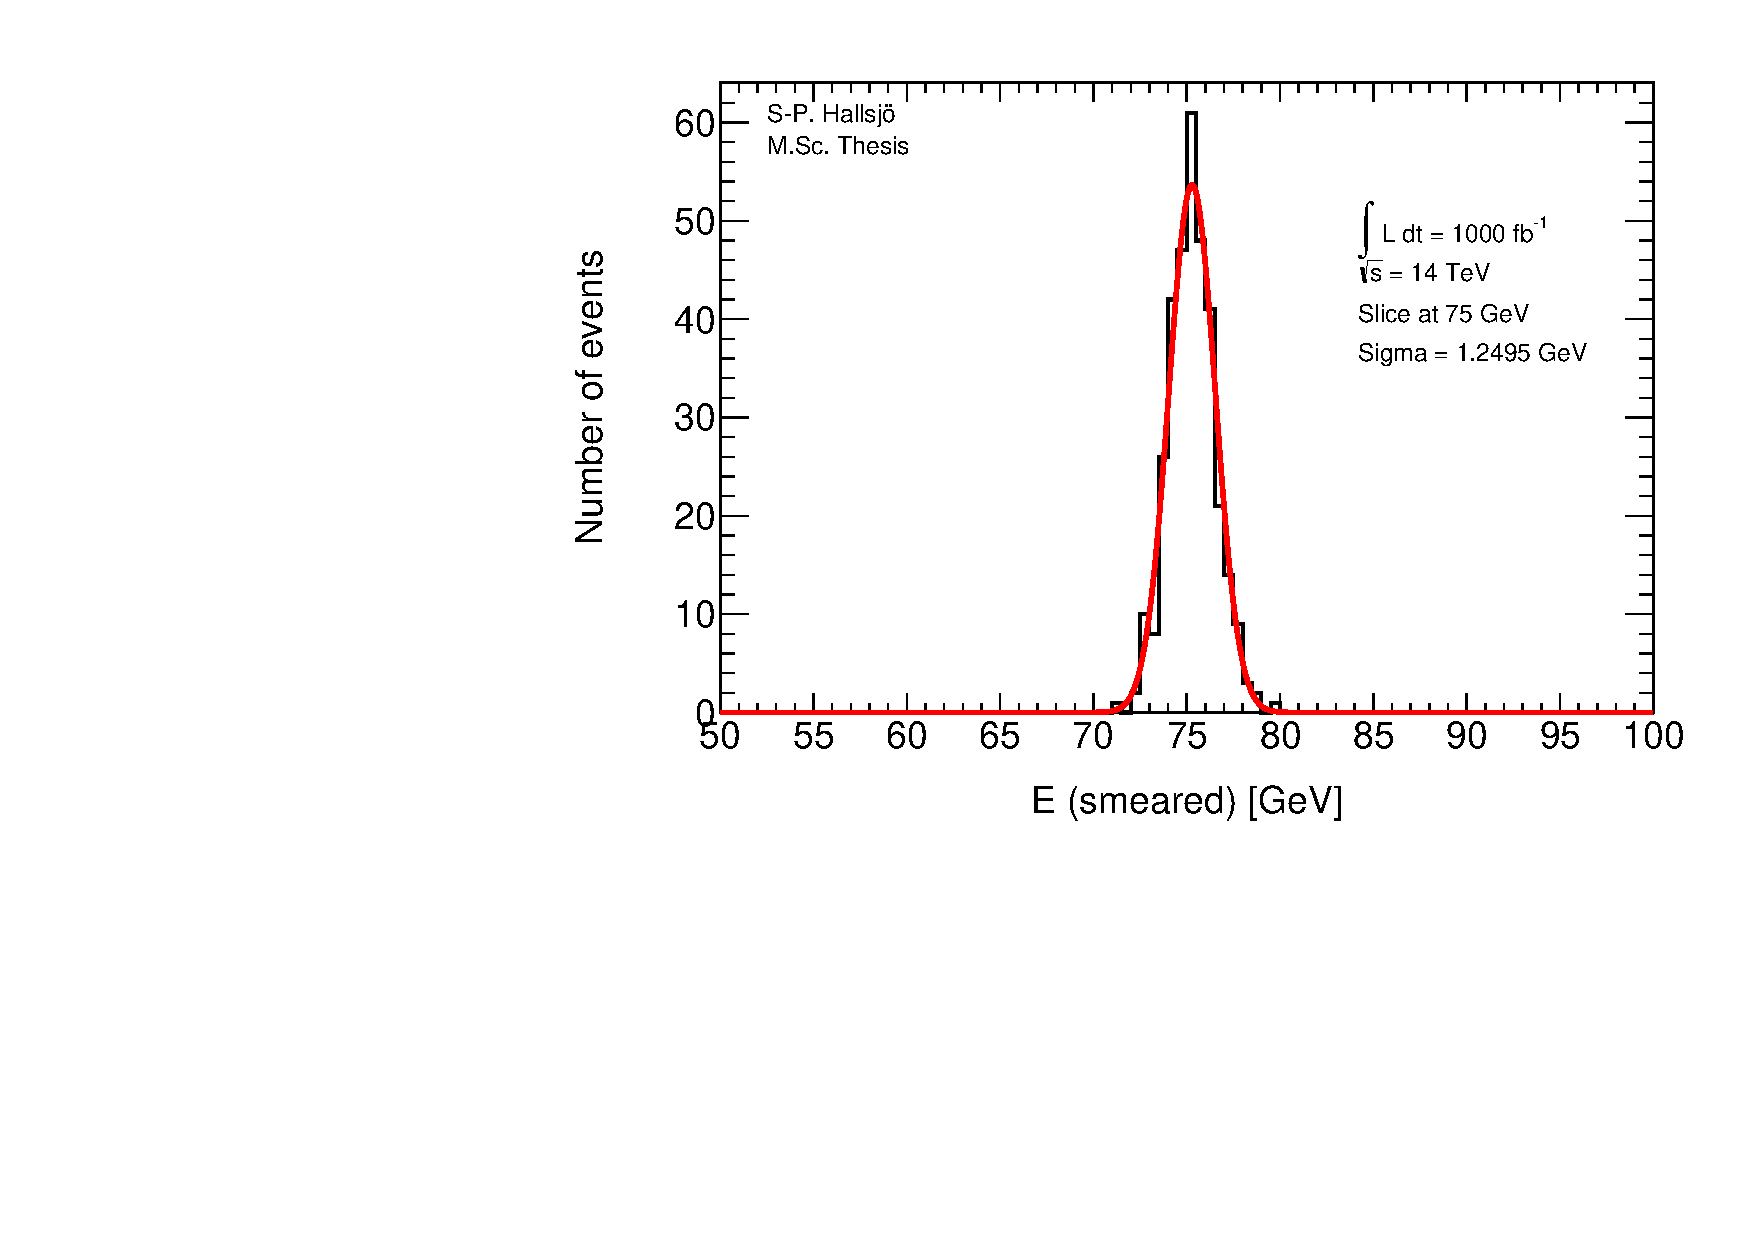
\includegraphics[width=0.5\textwidth]{eleta1.pdf}}% 
%\hfill
%  \subfloat[eleta2.\label{fig:elph:2}]{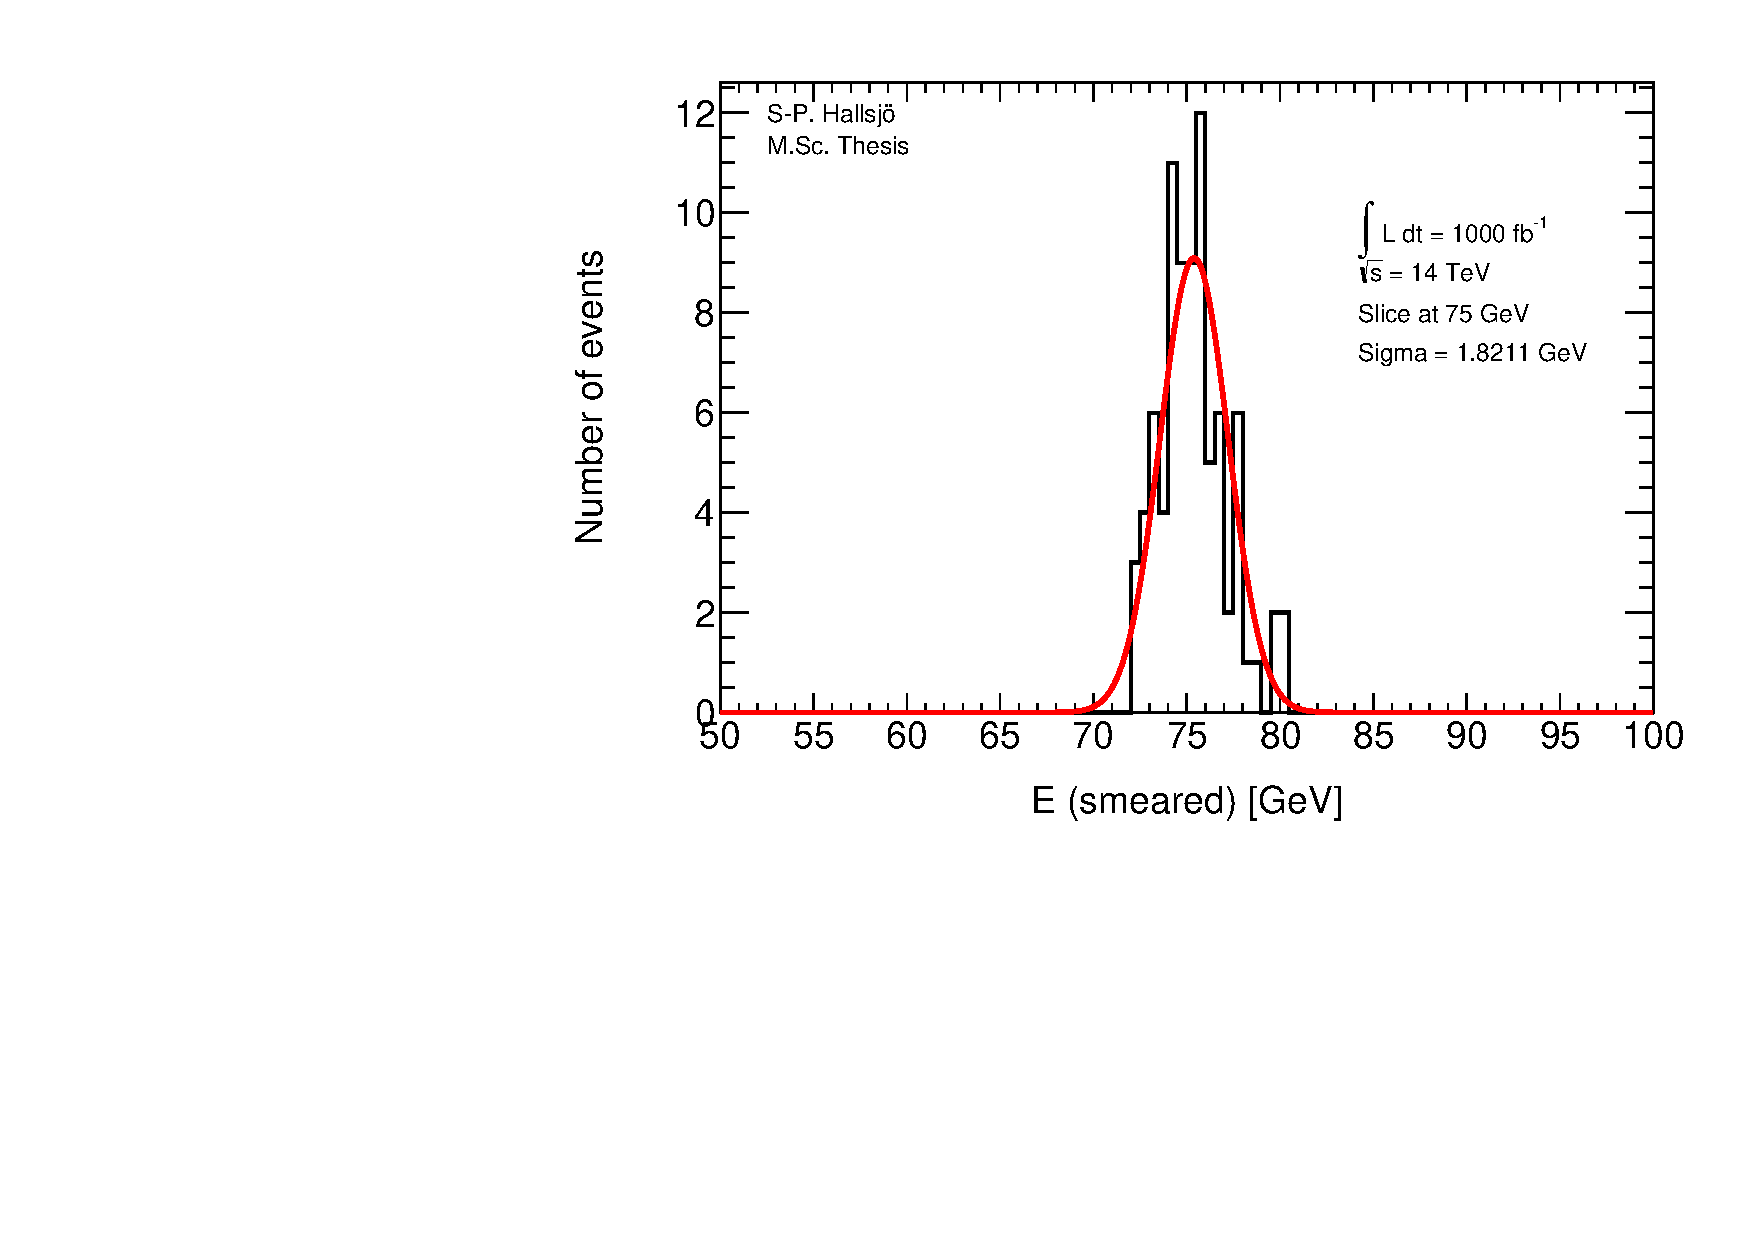
\includegraphics[width=0.5\textwidth]{eleta2.pdf}} 
%  \caption{el and ph eta}
%  \label{fig:elph}
%\end{figure}

%\begin{figure}[!htbp]
%% If it needs to be split.
%  \ContinuedFloat 
%  \centering 
%  \subfloat[pheta1. \label{fig:elph:3}]{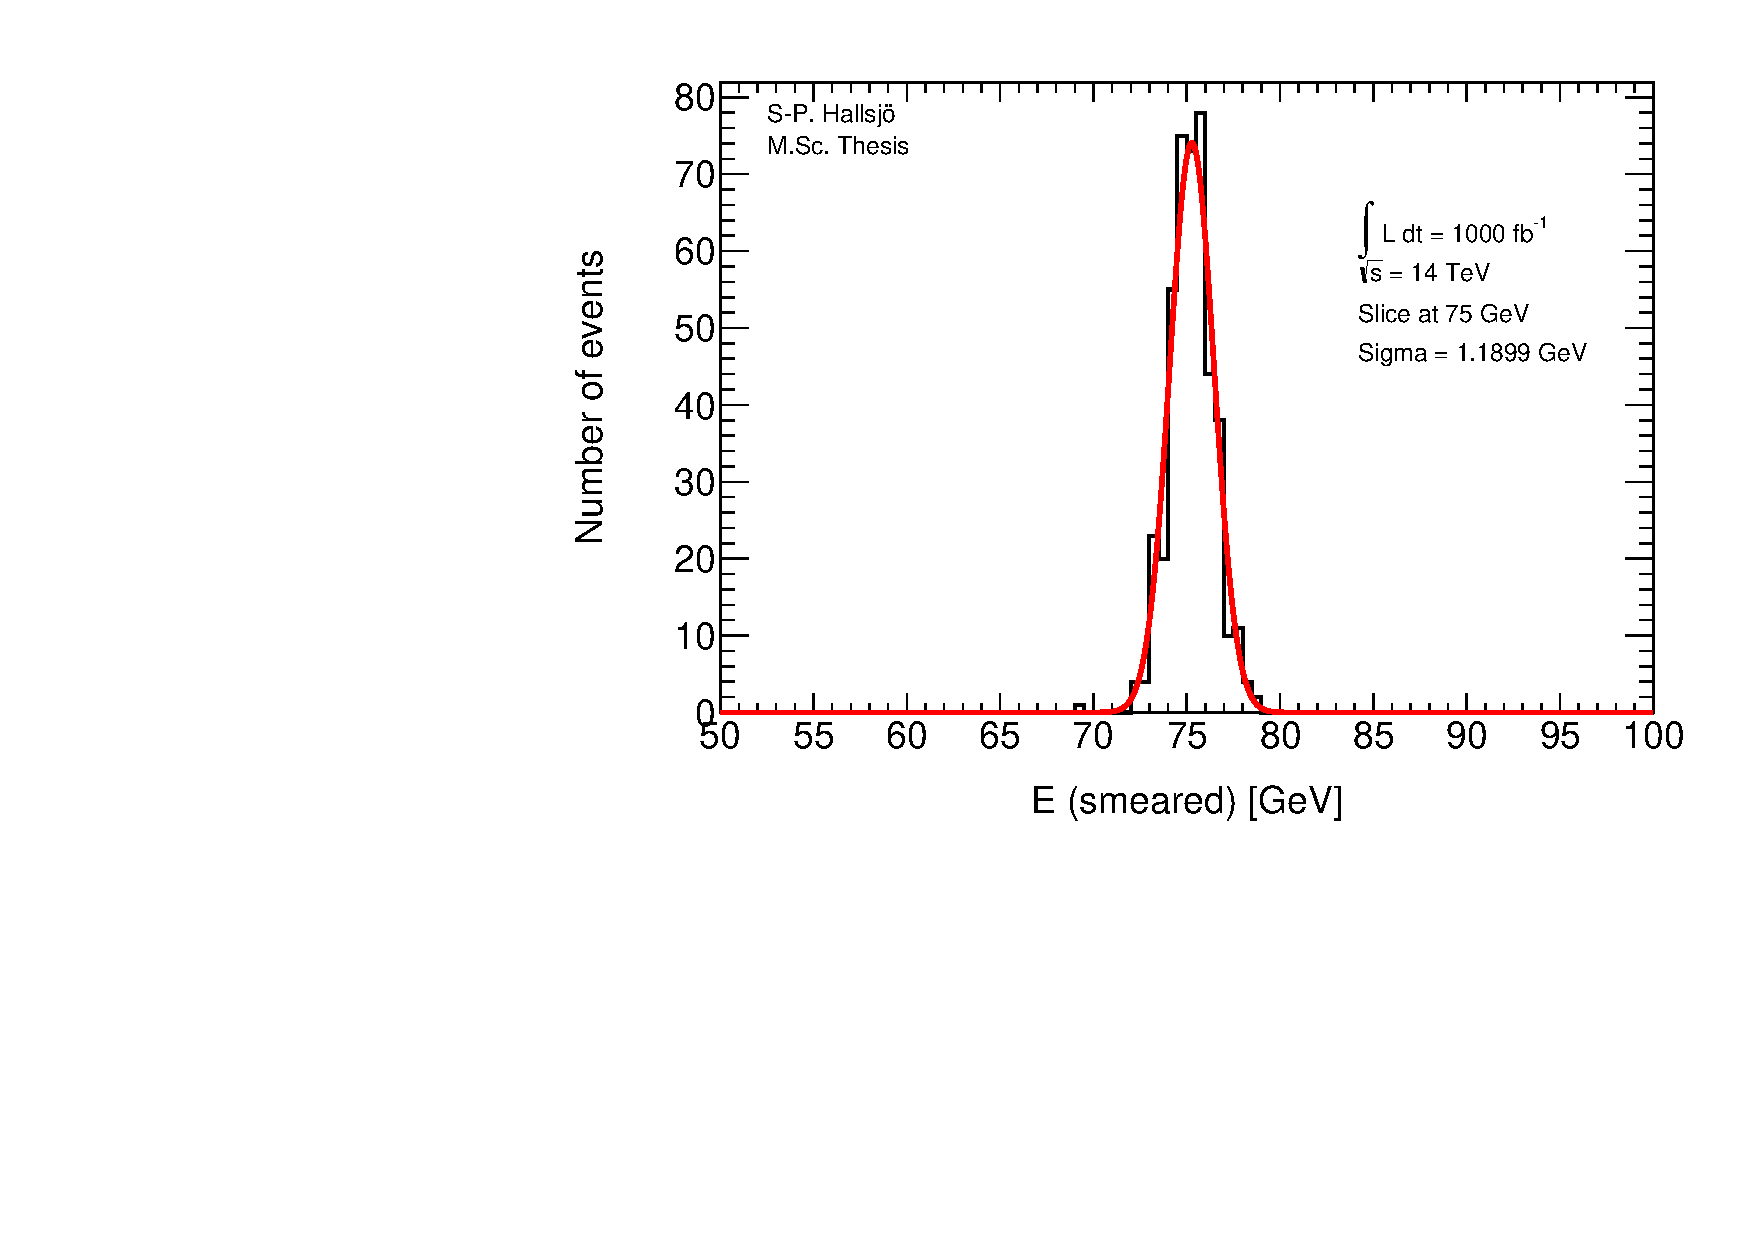
\includegraphics[width=0.5\textwidth]{pheta1.pdf}}% 
%  \hfill
%  \subfloat[pheta2.\label{fig:elph:4}]{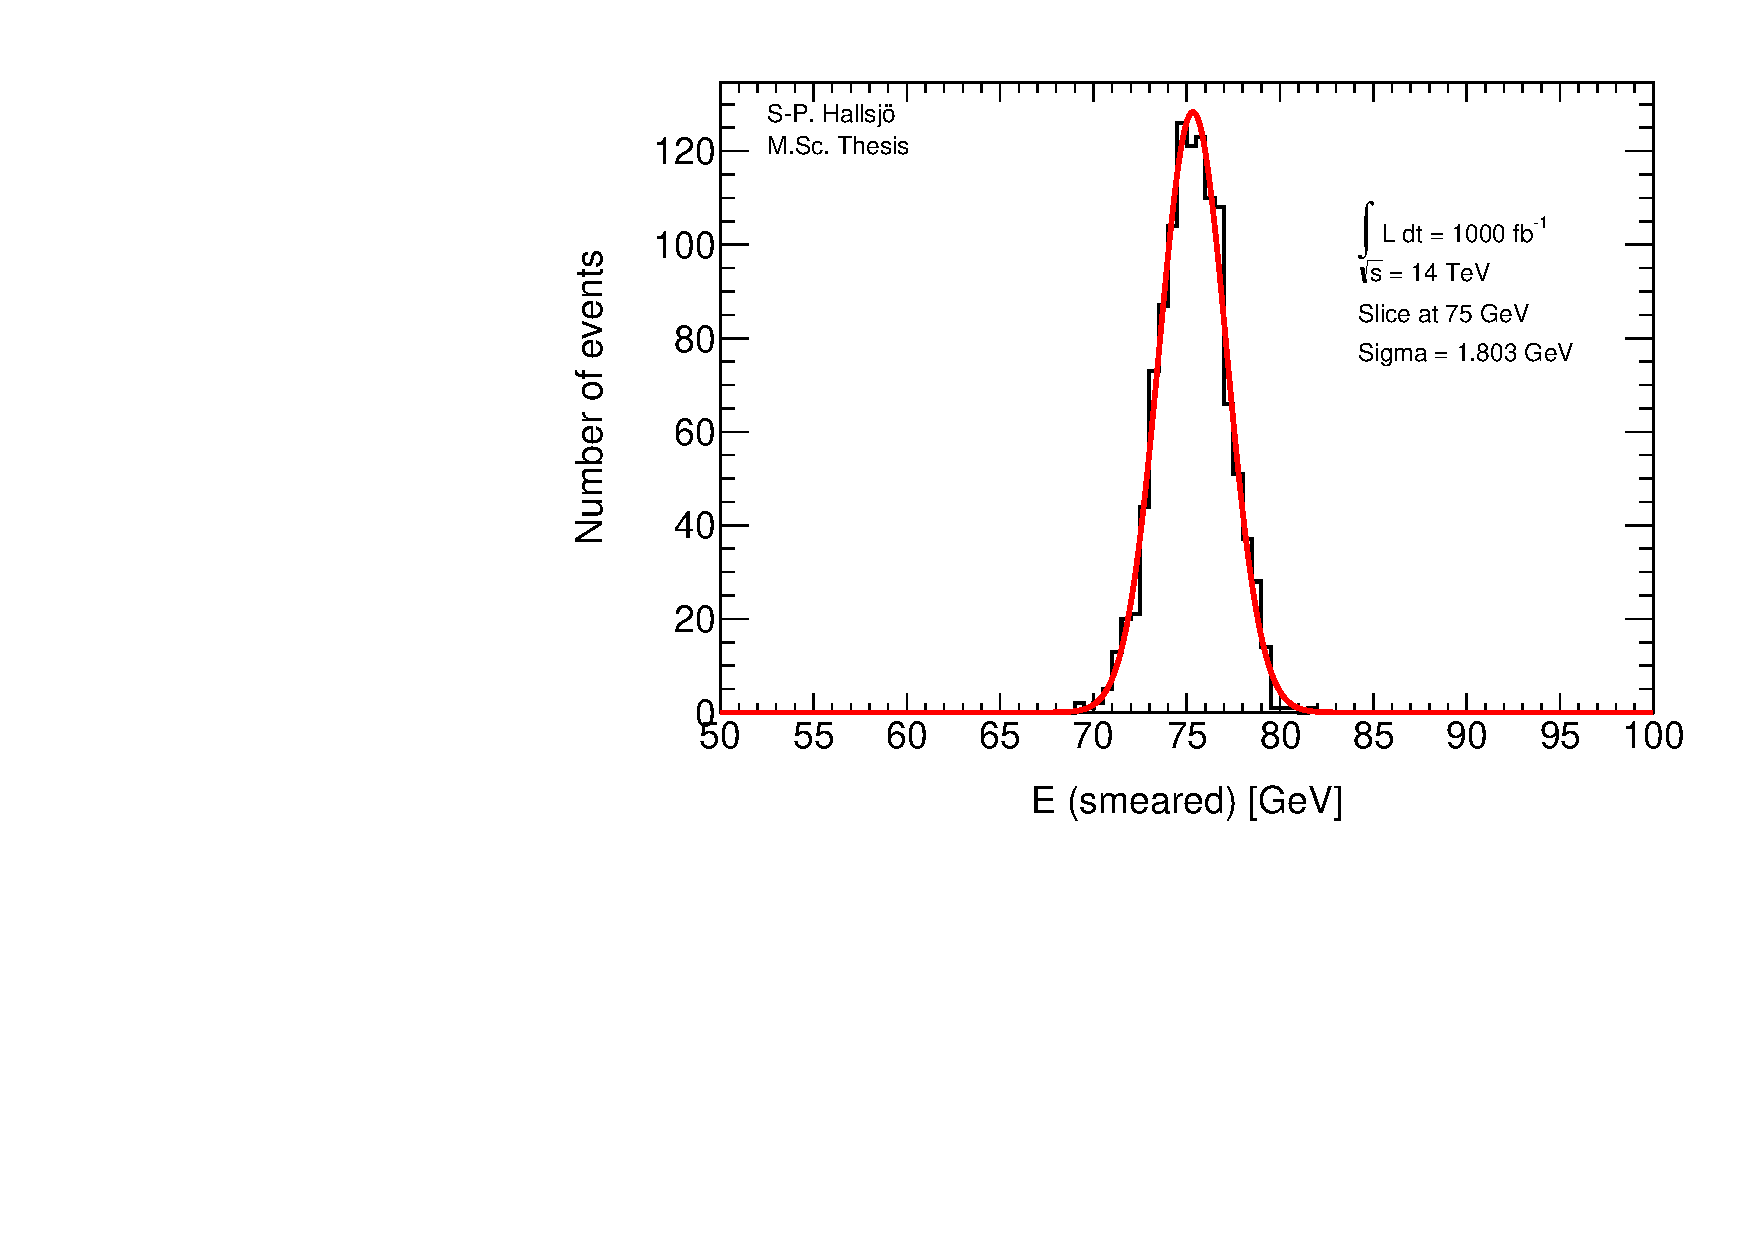
\includegraphics[width=0.5\textwidth]{pheta2.pdf}} 
%  \setcounter{figure}{1}
%  \caption[]{el and ph eta}
%  \label{fig:elph}
%\end{figure} 
%\setcounter{figure}{1}

 \begin{figure}[H] %!ht
    \subfloat[Electron smearing for $\abs{\eta}<1.4$. \label{fig:elph:1}]{%
    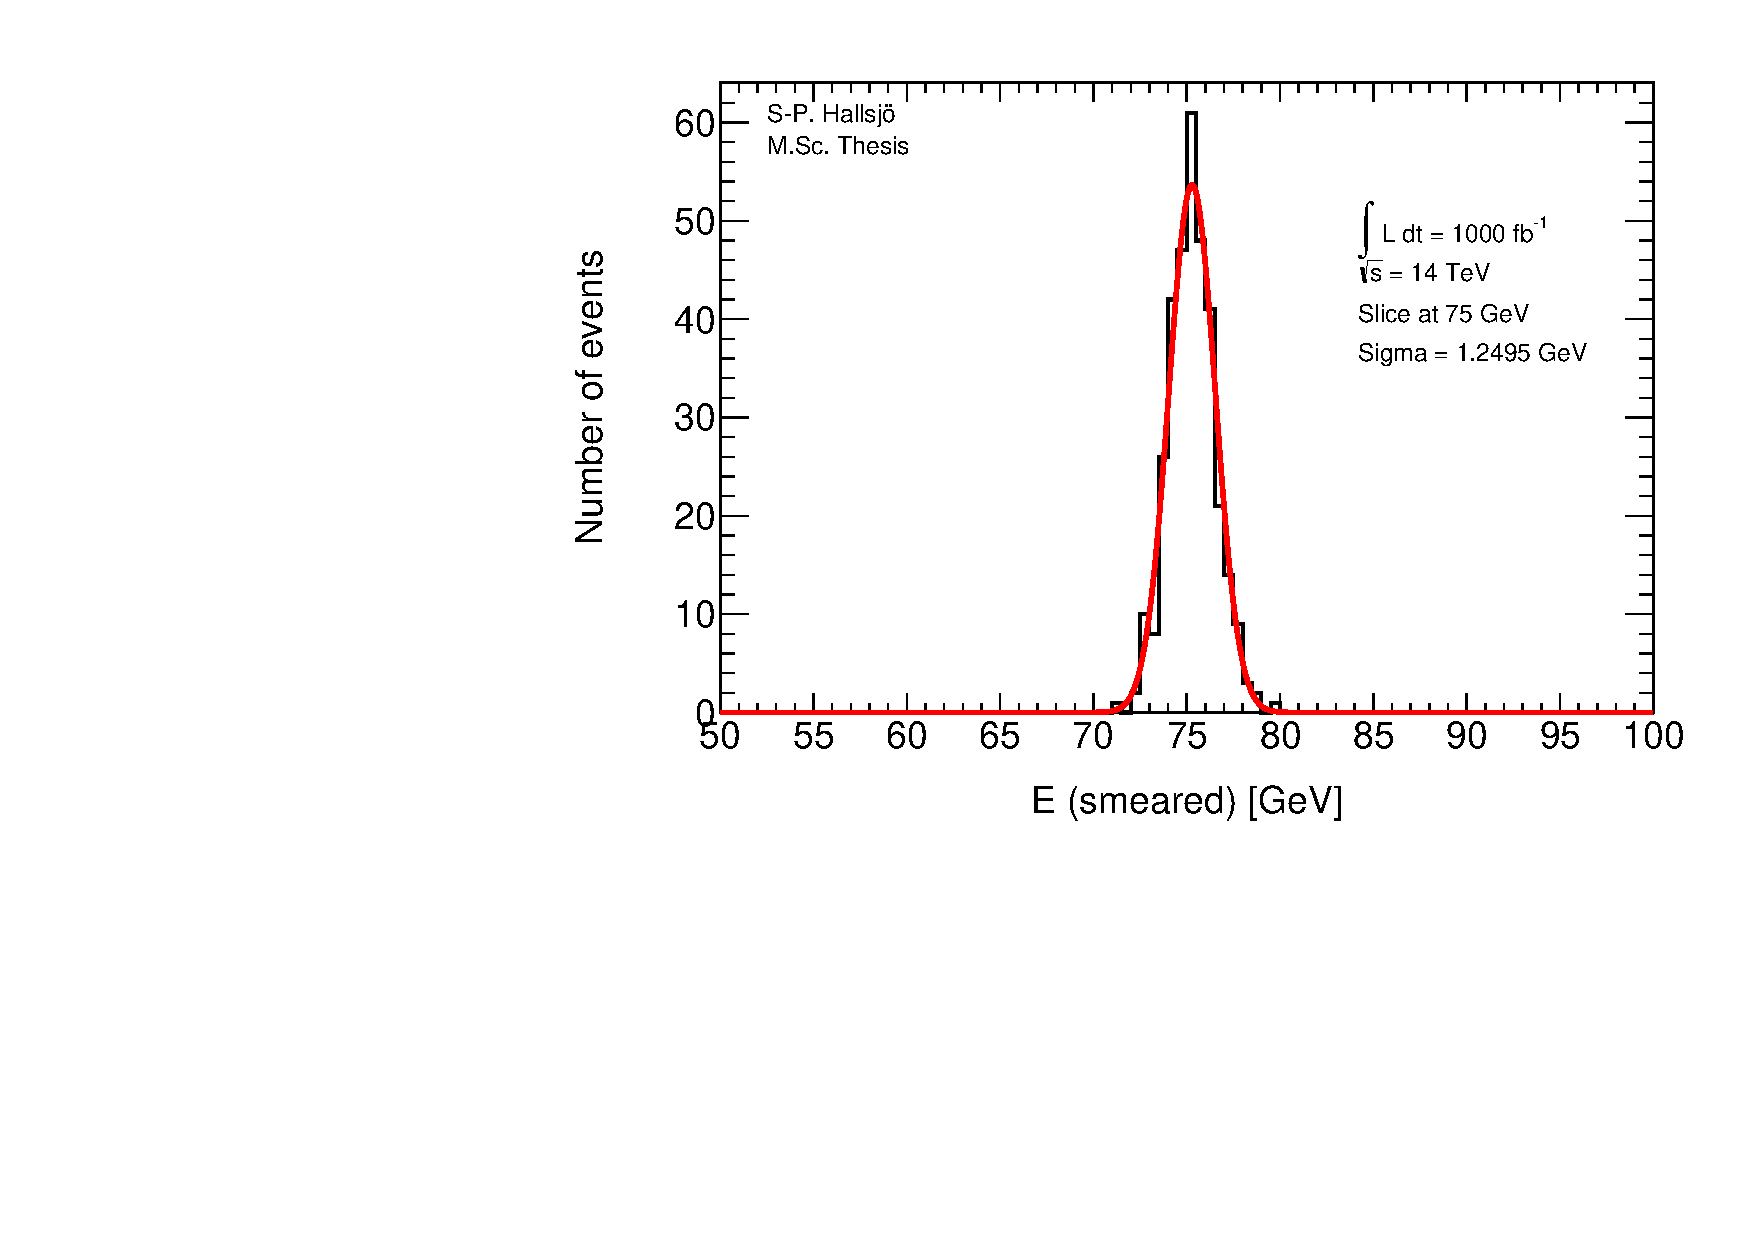
\includegraphics[width=0.5\textwidth]{eleta1.pdf}
    }
    \hfill
\subfloat[Electron smearing for $1.4<\abs{\eta}<2.47$.\label{fig:elph:2}]{%
      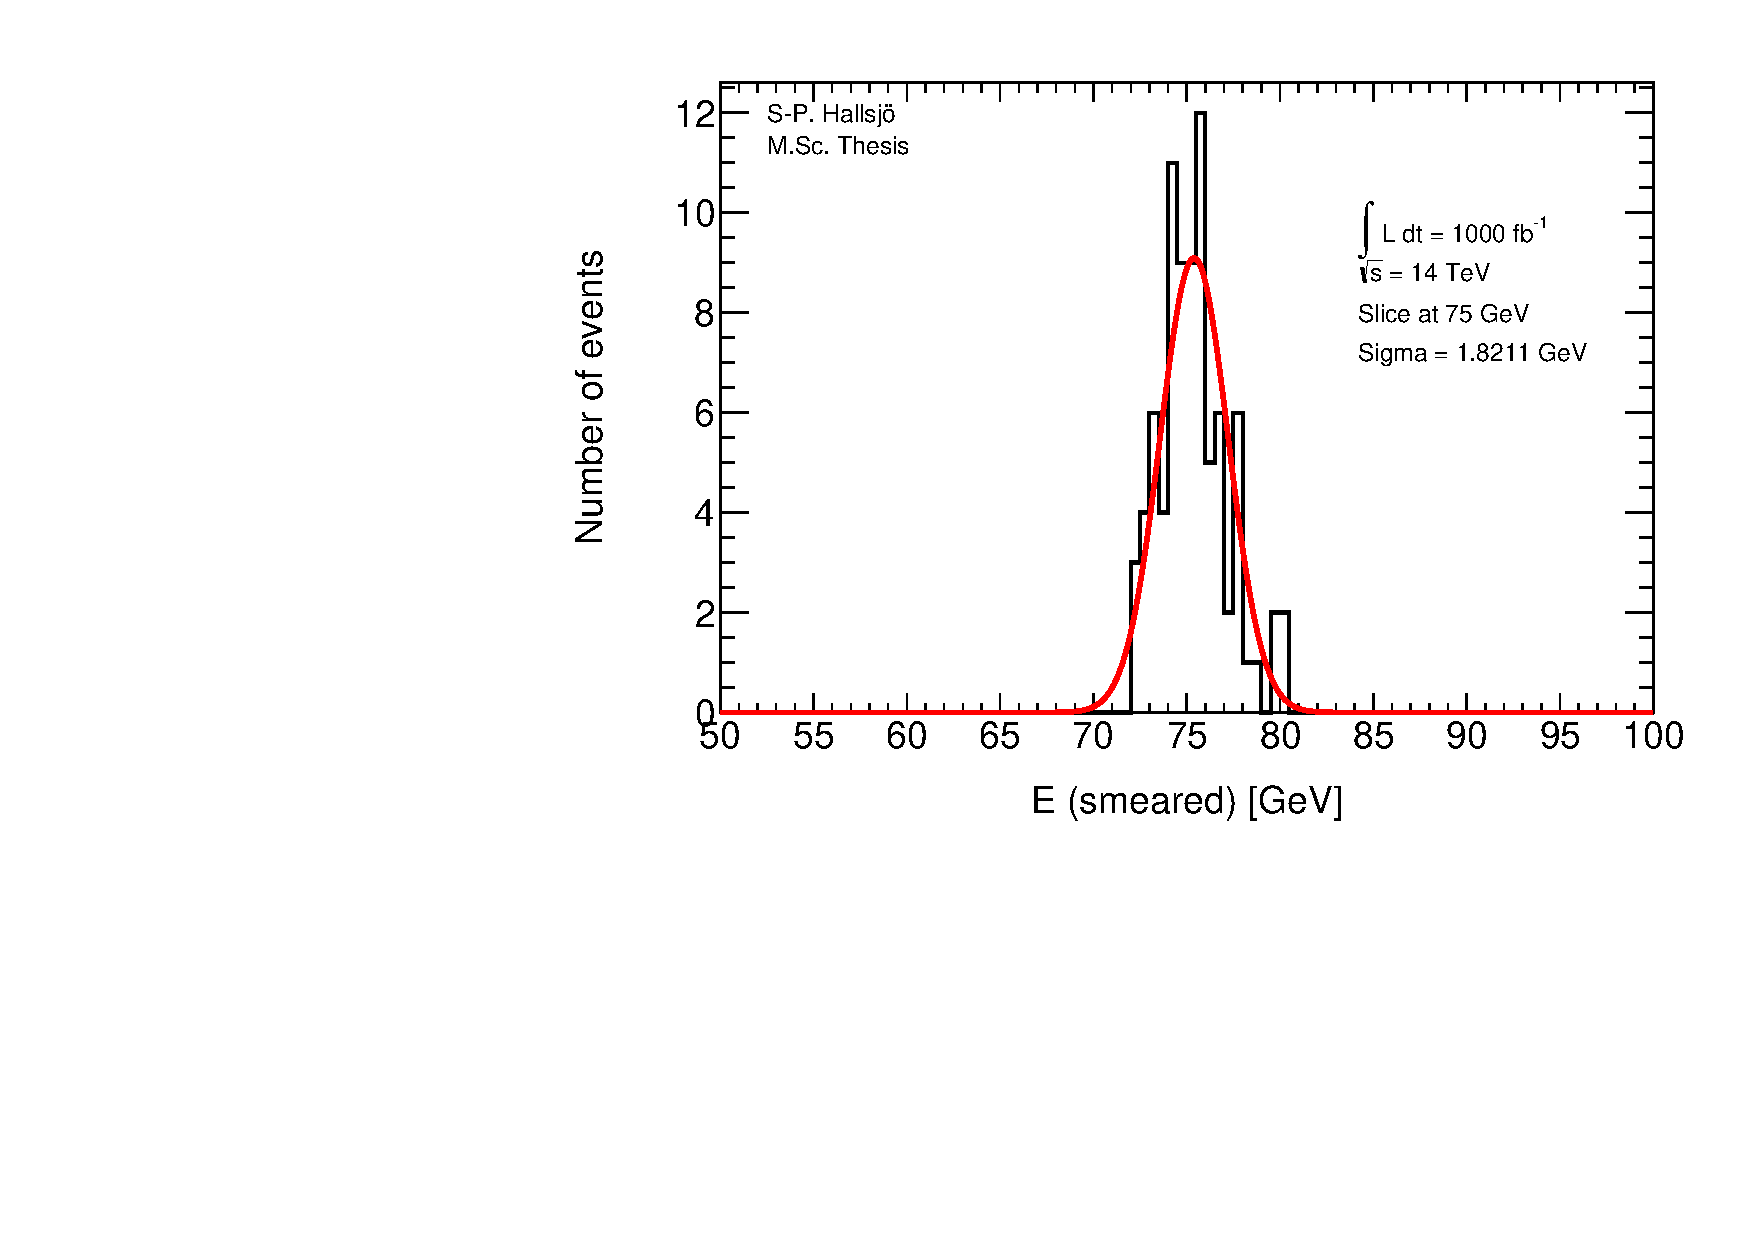
\includegraphics[width=0.5\textwidth]{eleta2.pdf}
    }
    \hfill
        \subfloat[Photon smearing for $\abs{\eta}<1.4$. \label{fig:elph:3}]{%
     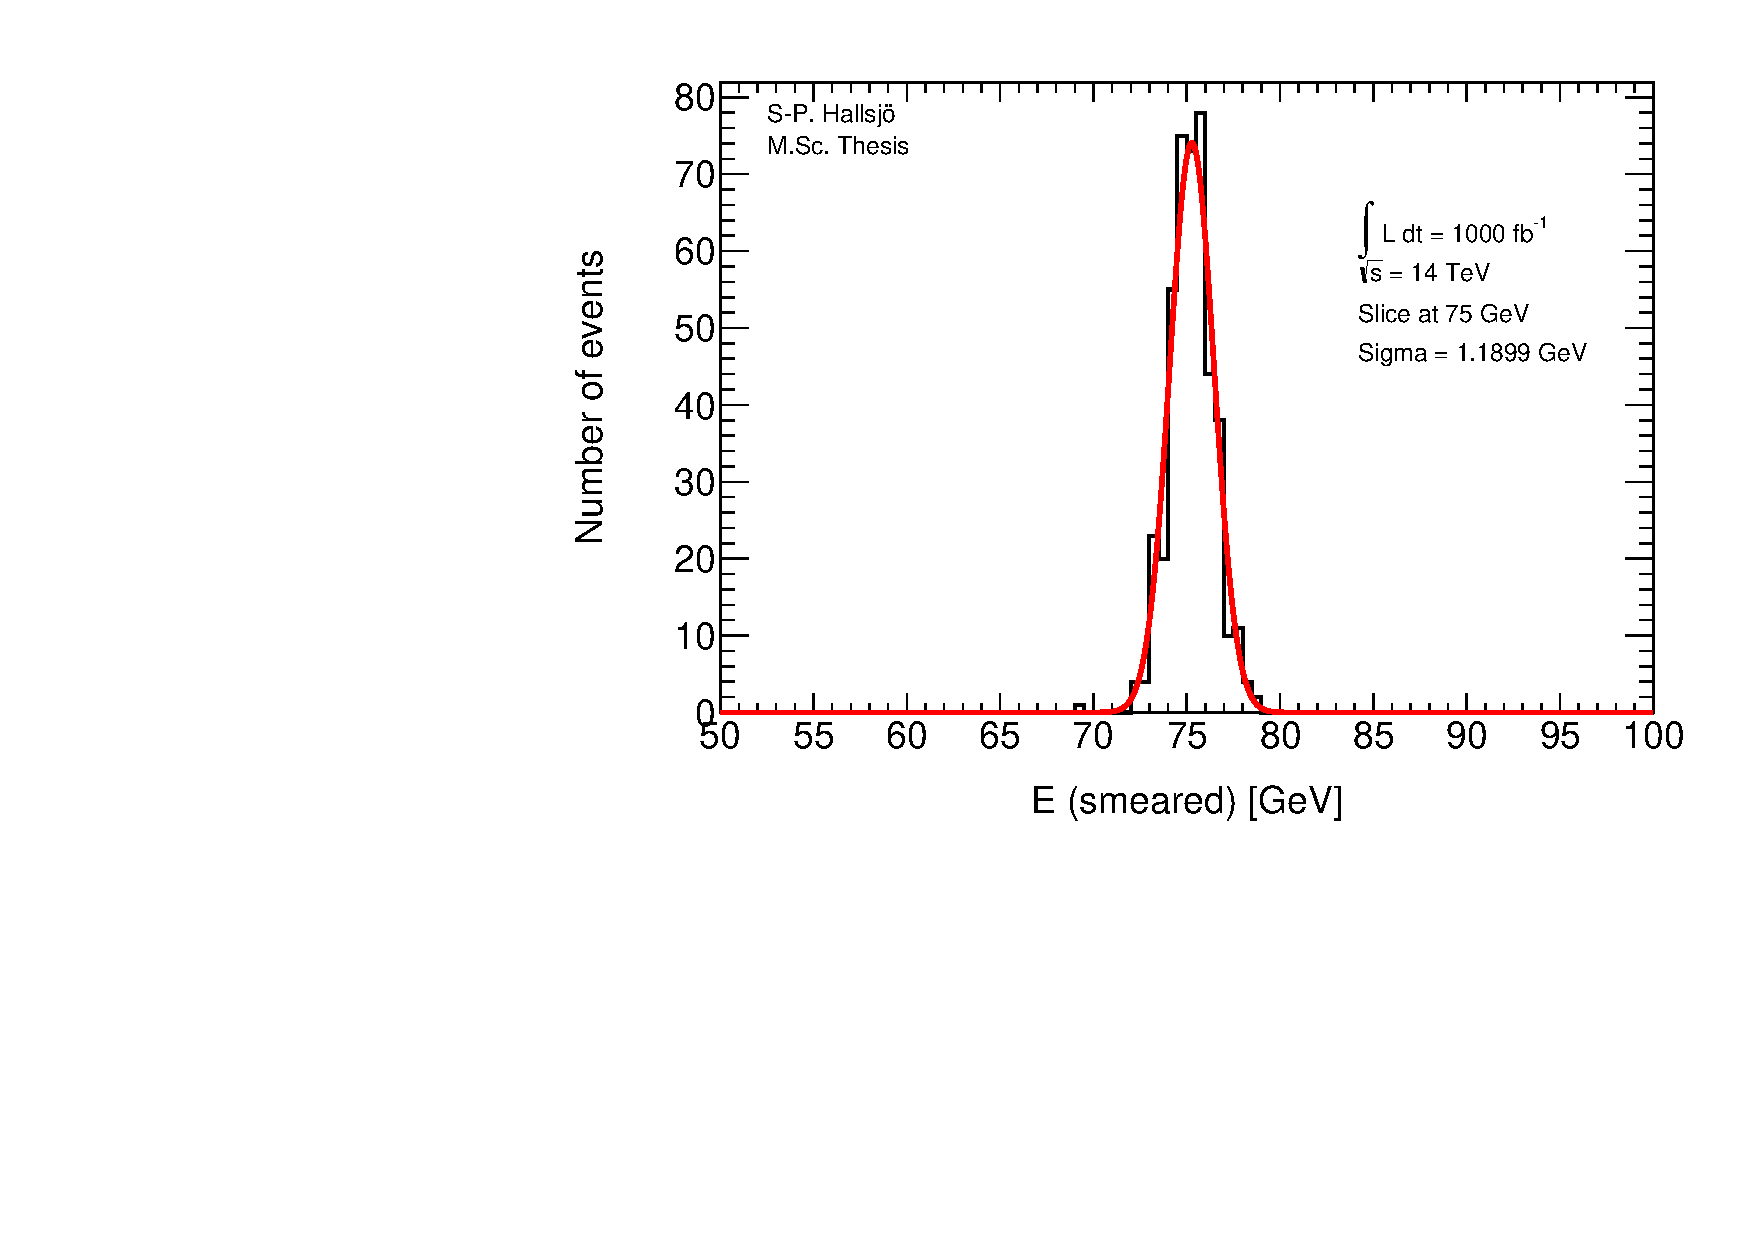
\includegraphics[width=0.5\textwidth]{pheta1.pdf}
    }
    \hfill
\subfloat[Photon smearing for $1.4<\abs{\eta}<2.47$.\label{fig:elph:4}]{%
     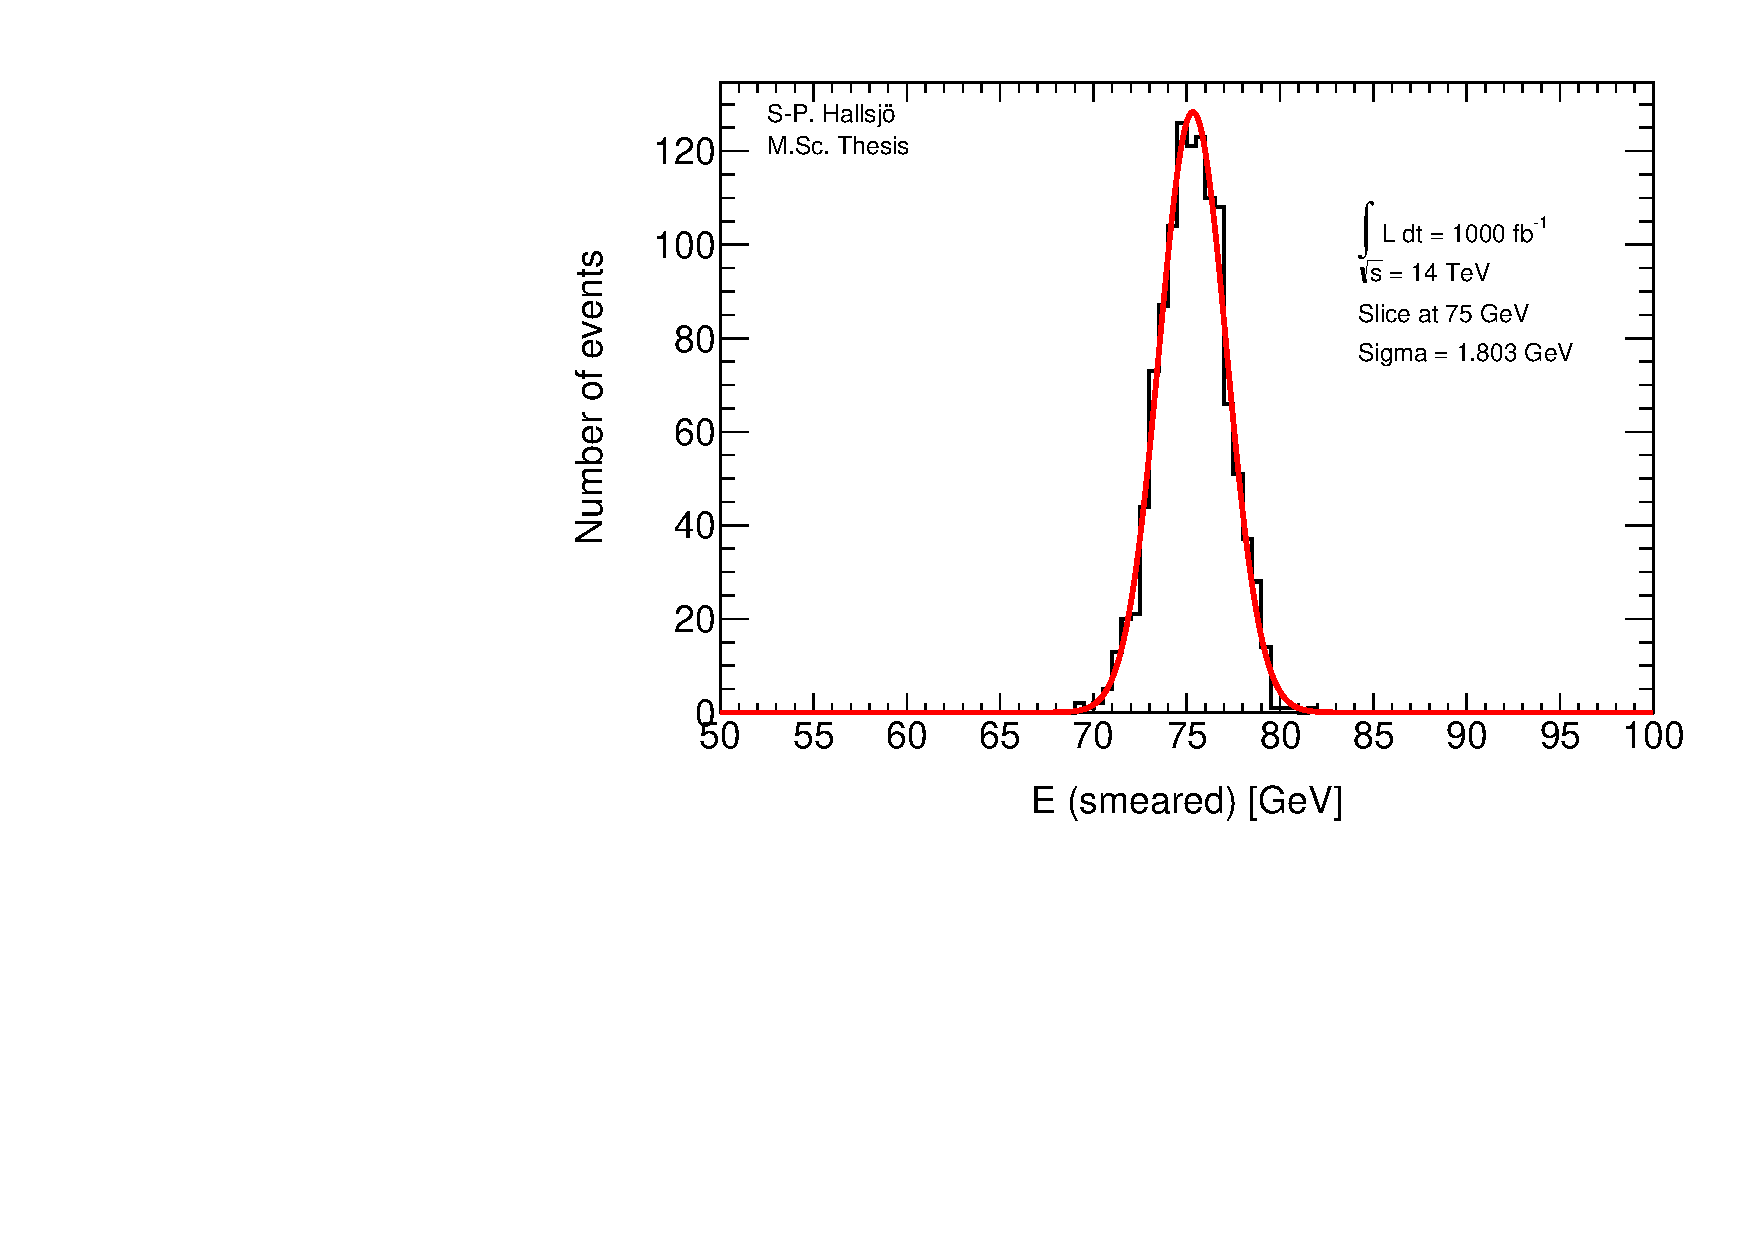
\includegraphics[width=0.5\textwidth]{pheta2.pdf}
    }
    \caption{Photon and electron smearing plots.}
    \label{fig:elph}
\end{figure}
\newpage
\subsection{Muon}
 \begin{figure}[H] %!ht
    \subfloat[Muon smearing for $\abs{\eta}<1.05$. \label{fig:muon:1}]{%
     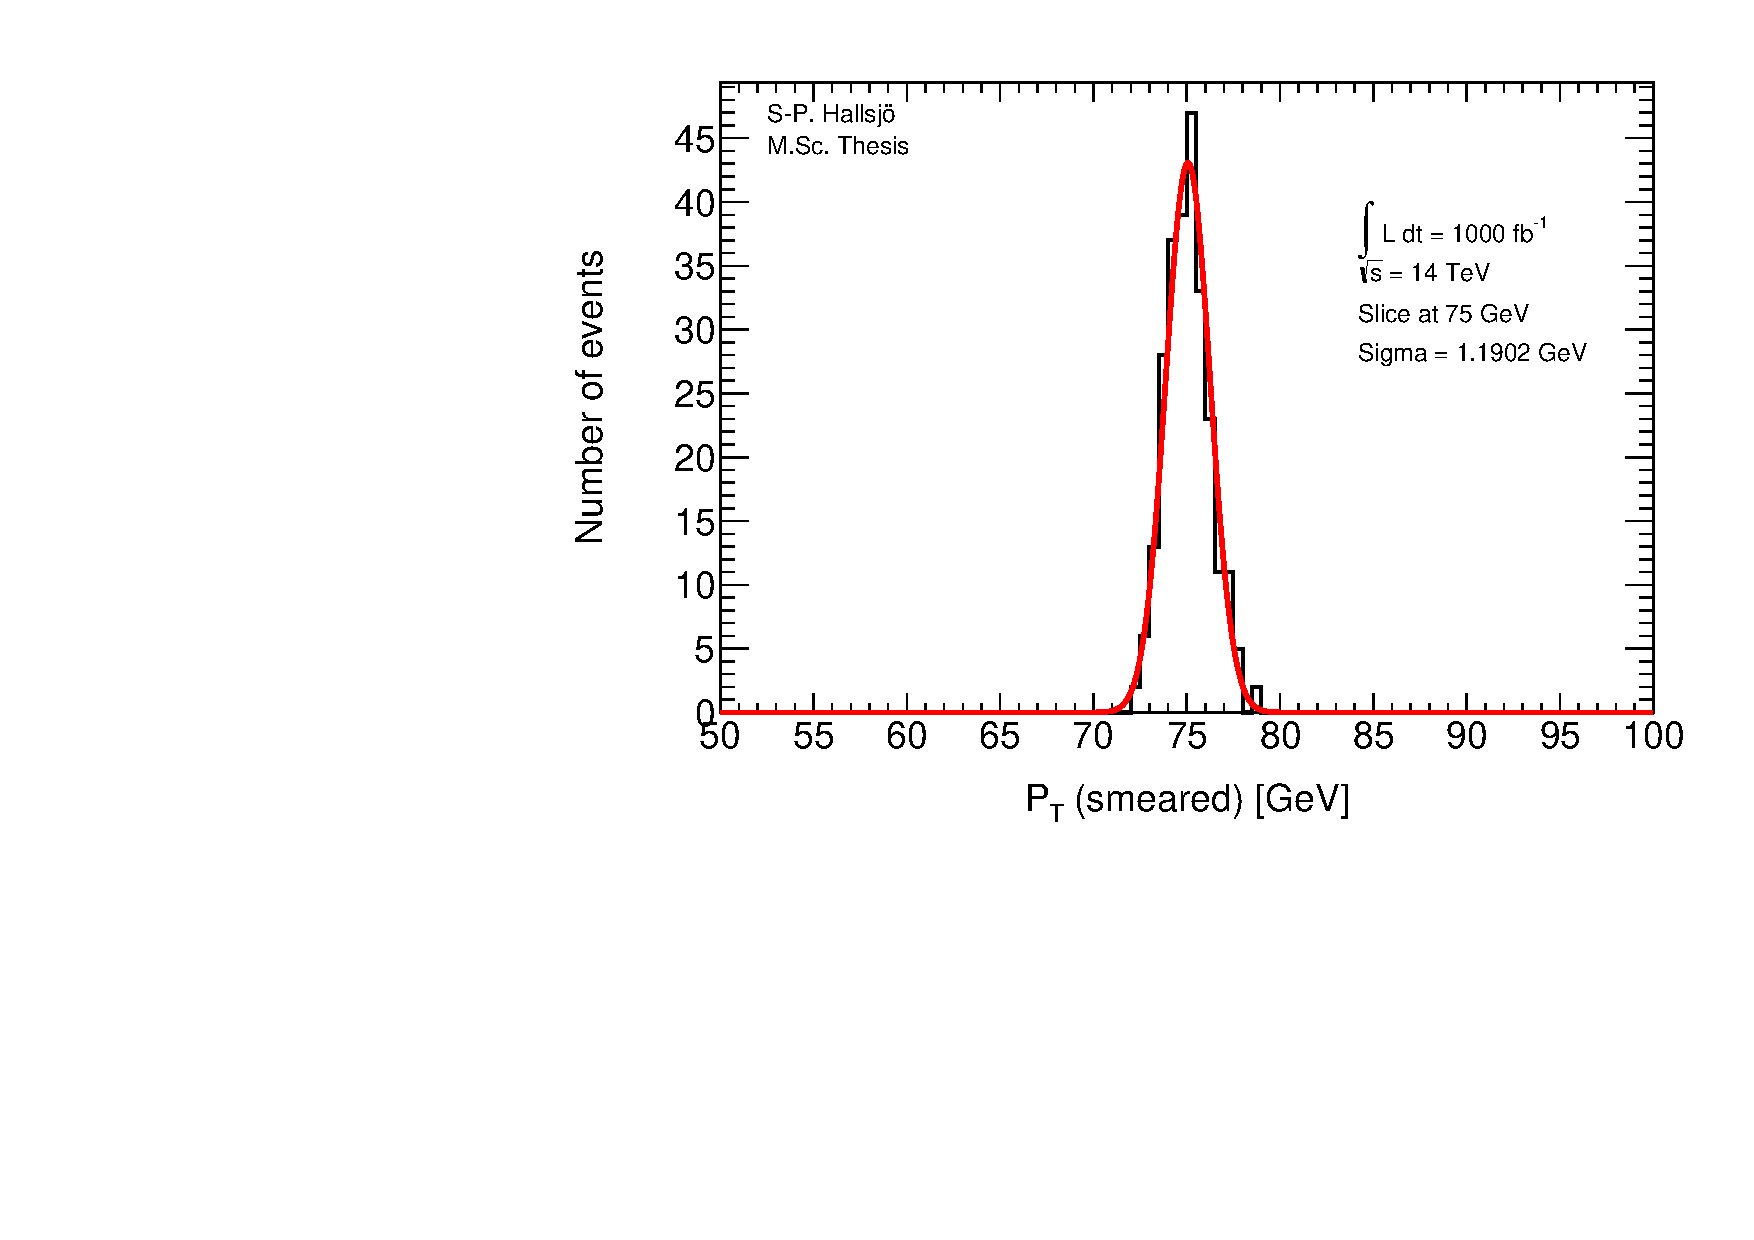
\includegraphics[width=0.5\textwidth]{mueta1.pdf}
    }
    \hfill
    \subfloat[Muon smearing for $1.05<\abs{\eta}$.\label{fig:muon:2}]{%
      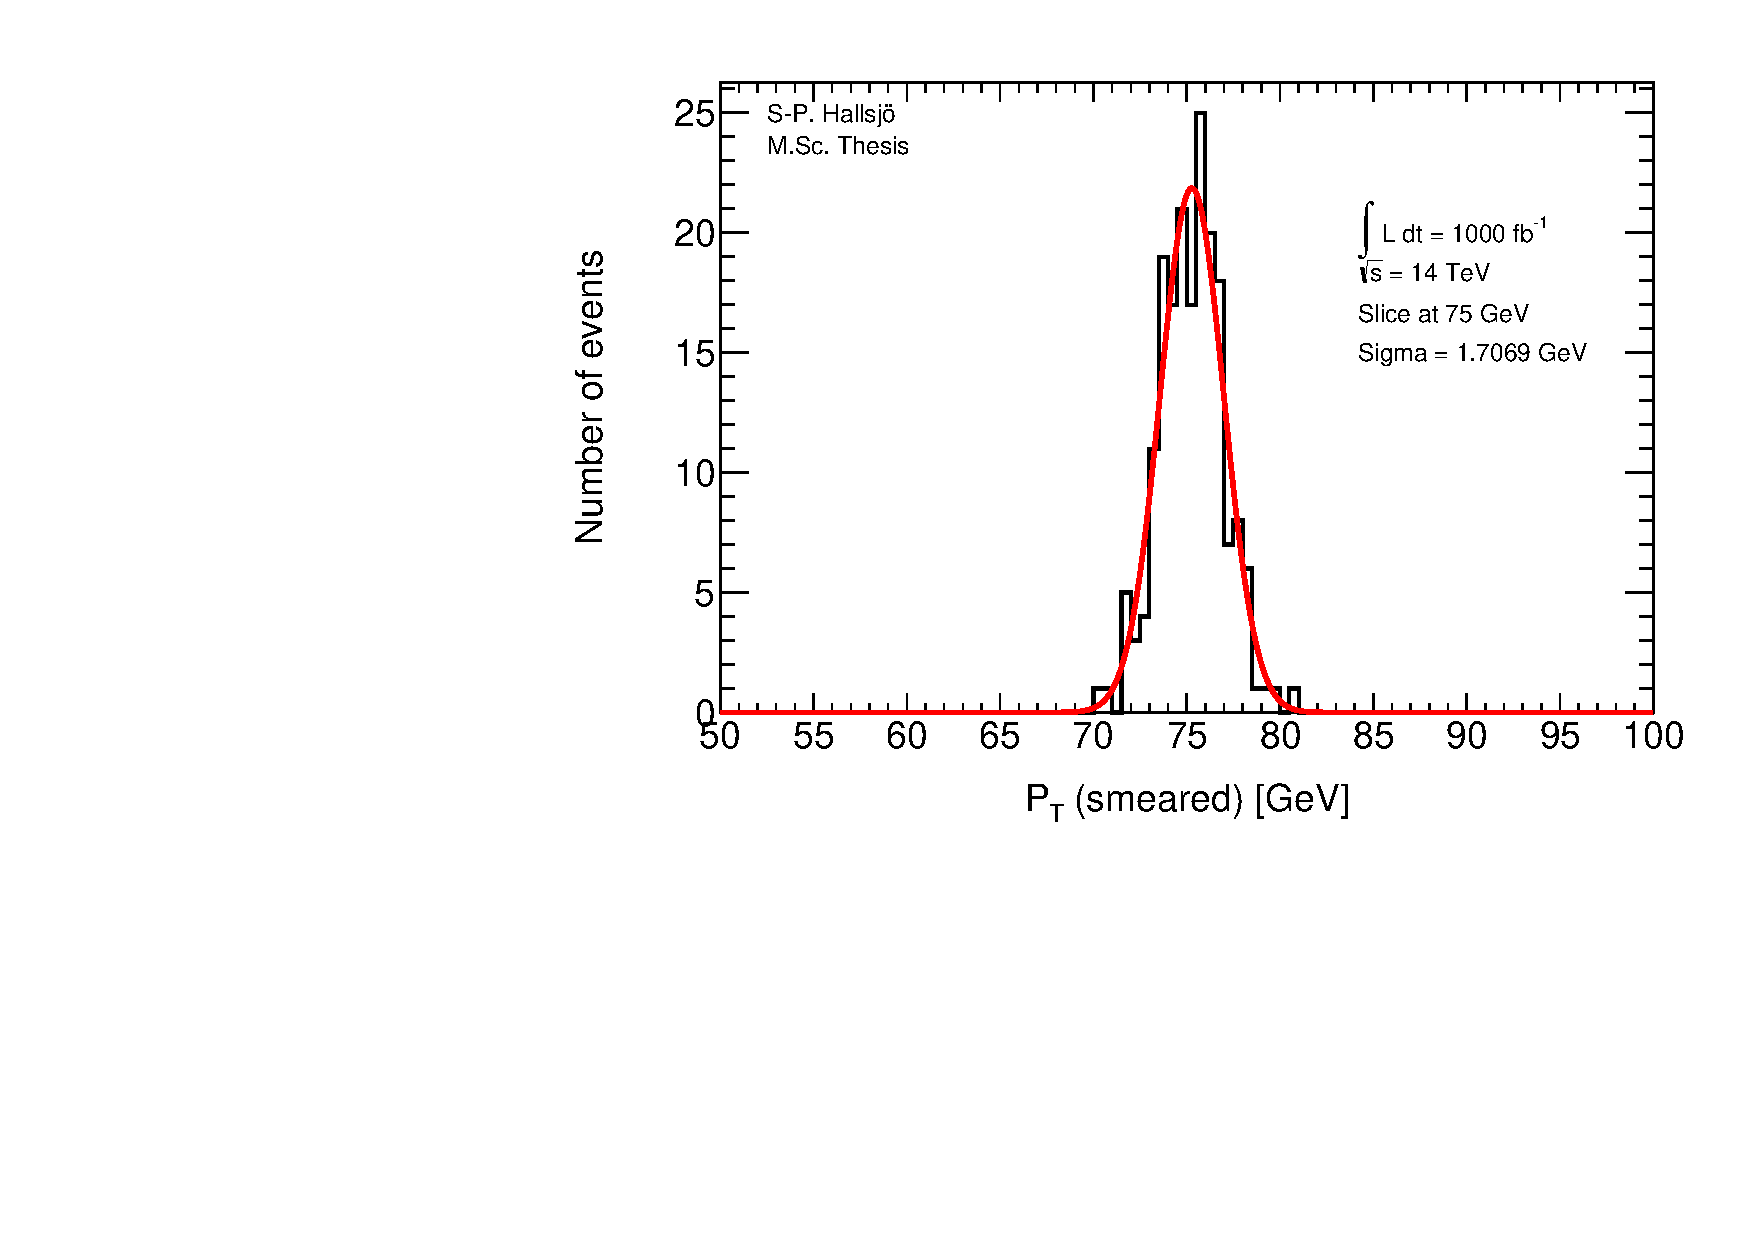
\includegraphics[width=0.5\textwidth]{mueta2.pdf}
    }
    \caption{Muon smearing plots.}
    \label{fig:muon}
  \end{figure}
\subsection{Tau}
 \begin{figure}[H] %!ht
    \subfloat[Tau smearing. \label{fig:tau:1}]{%
     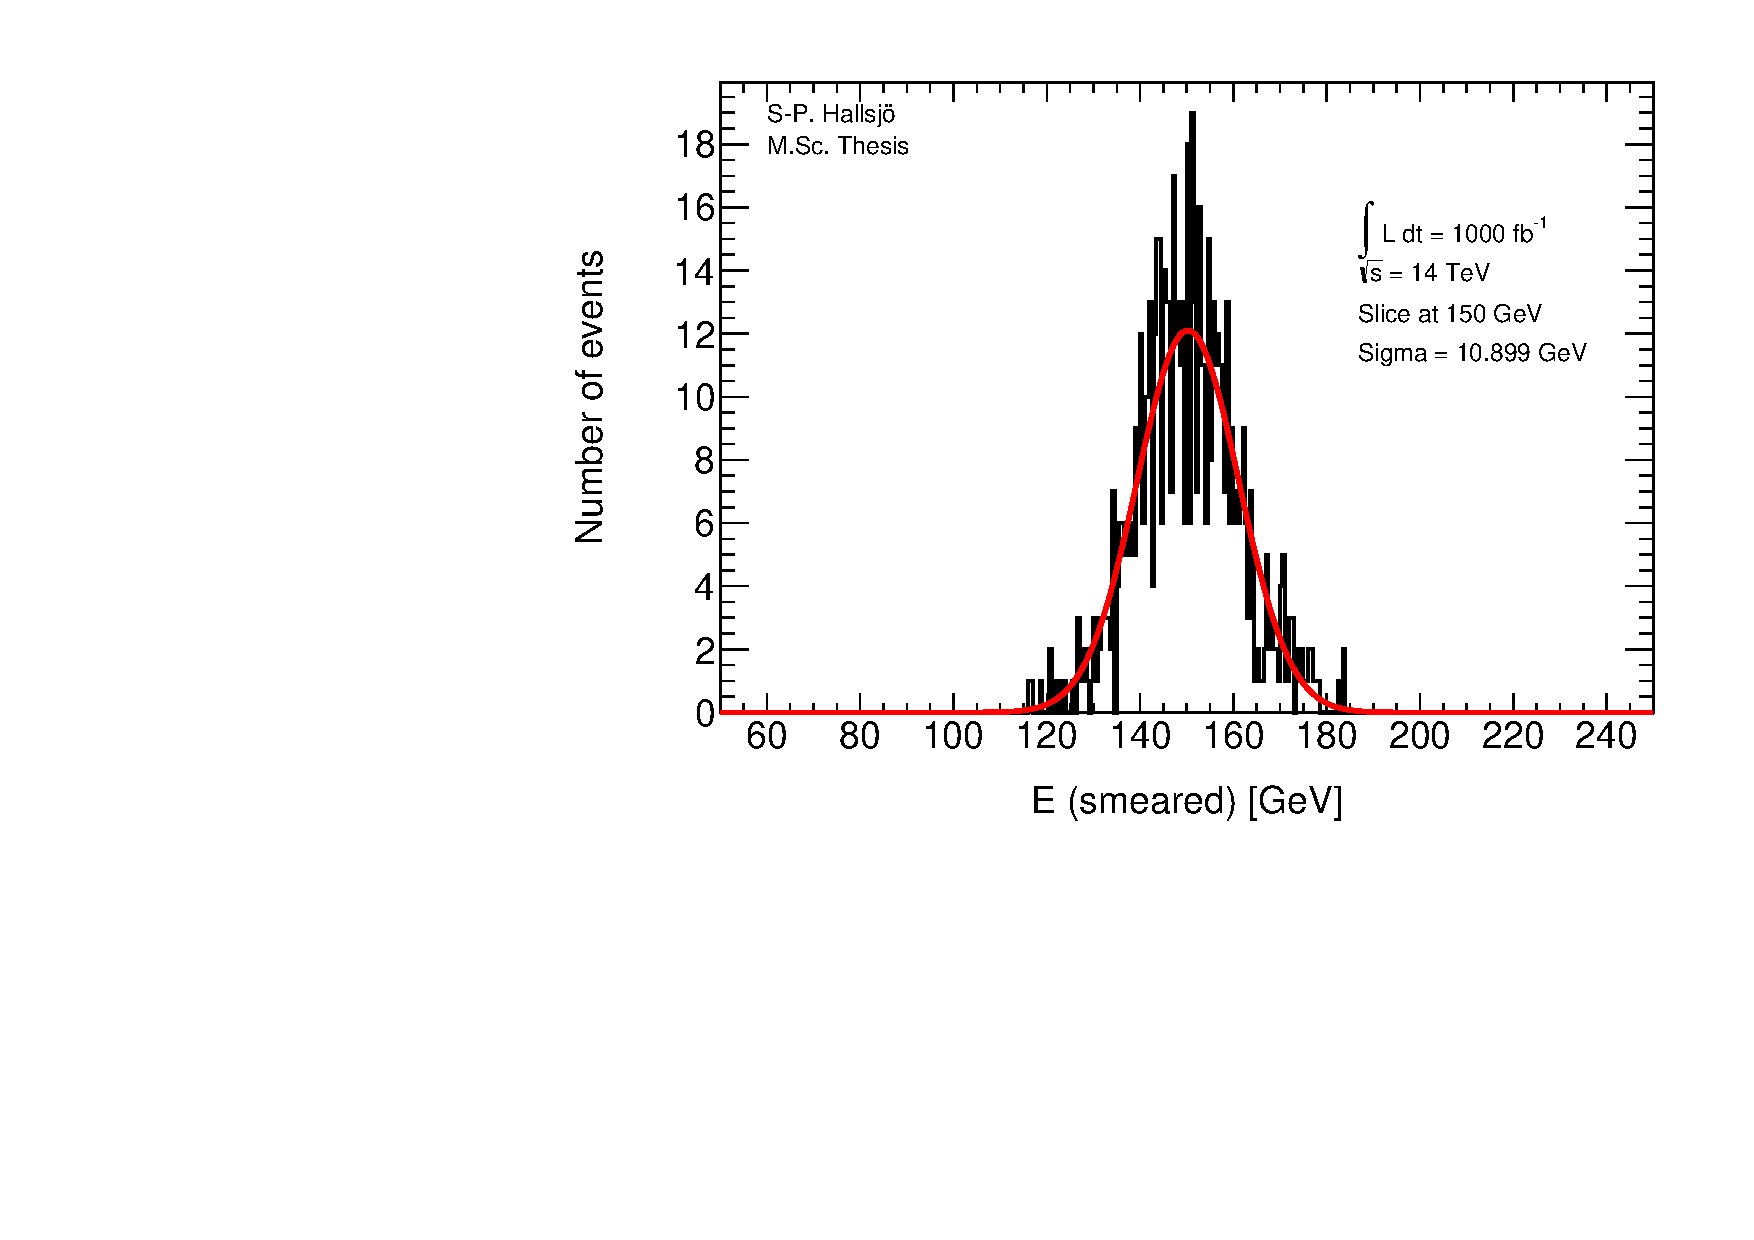
\includegraphics[width=0.5\textwidth]{tau.pdf}
    }
    \hfill
    \subfloat[Tau energy vs smeared. \label{fig:tau:2}]{%
      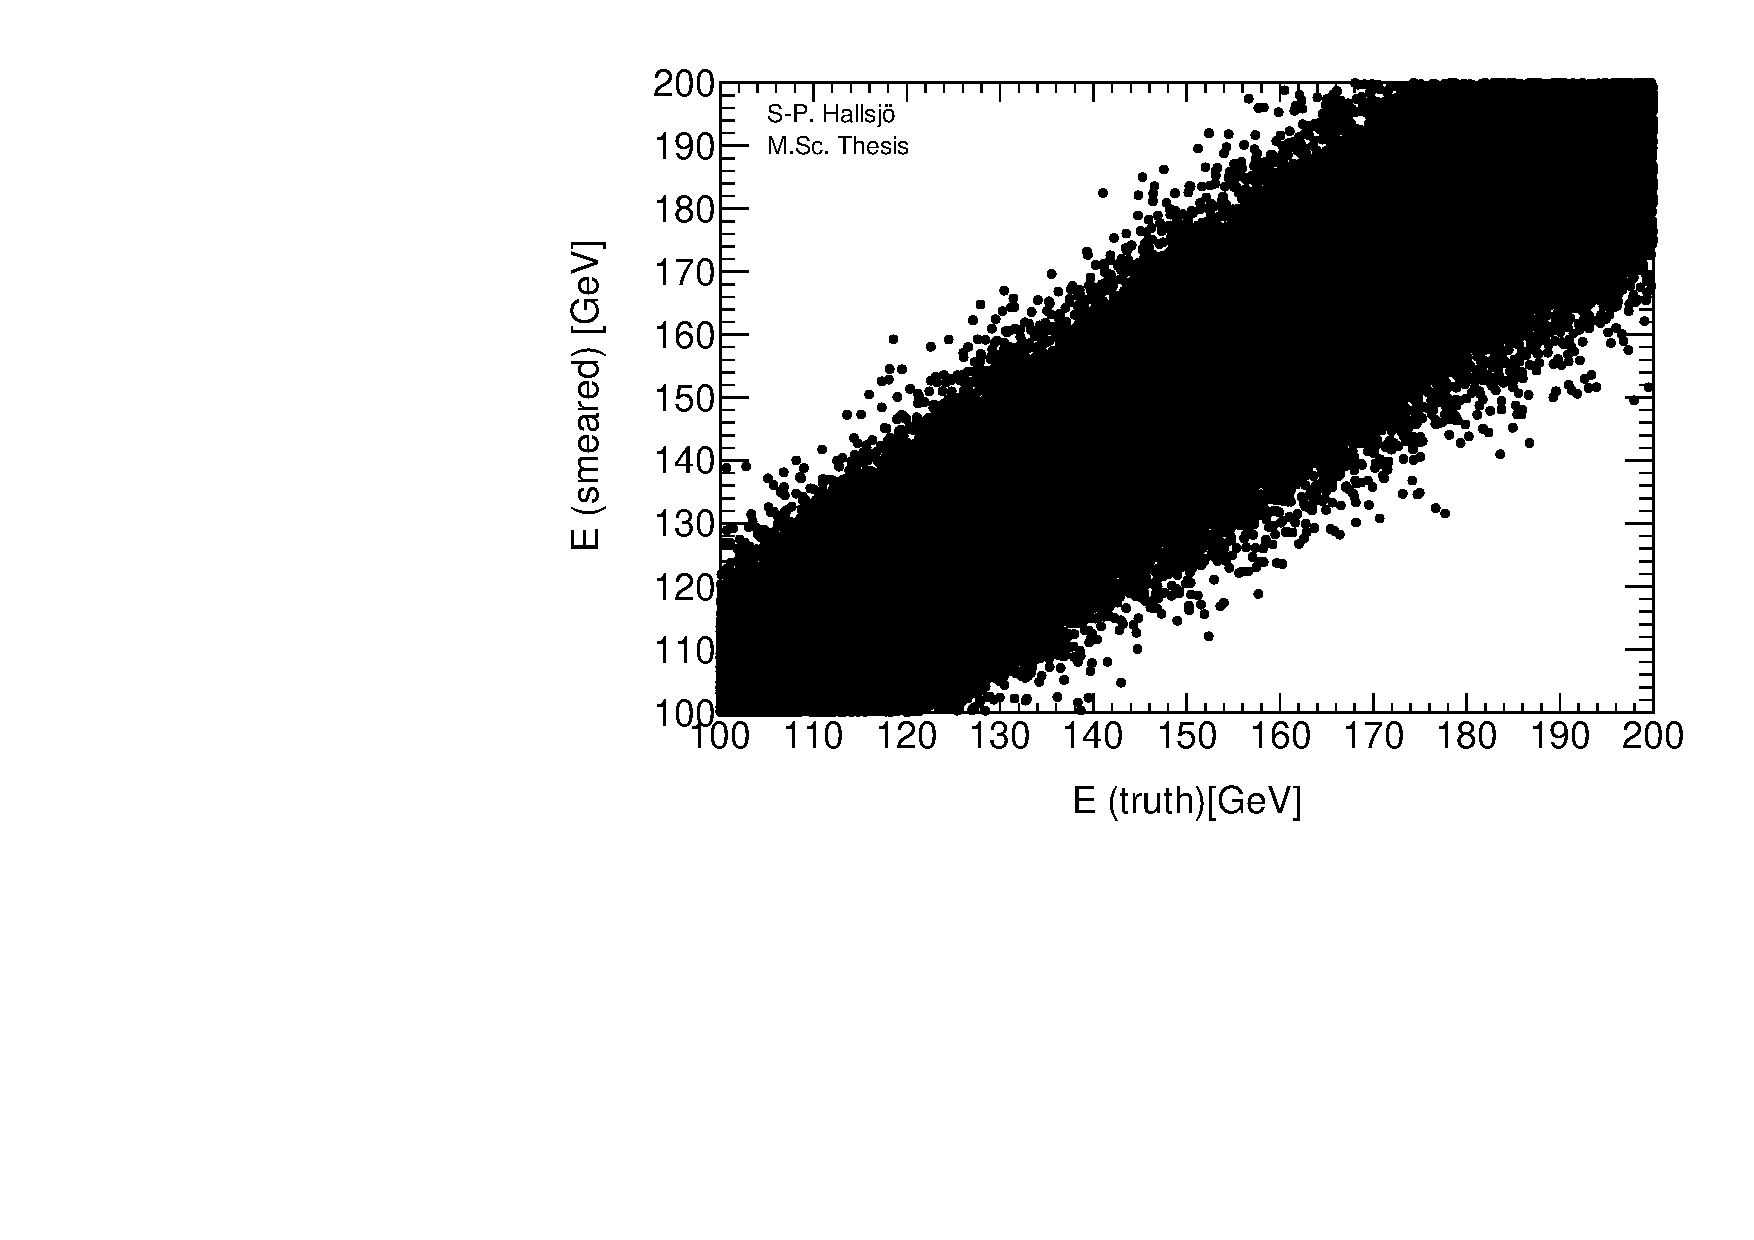
\includegraphics[width=0.5\textwidth]{tau2.pdf}
    }
    \caption{Tau smearing and energy vs smearing plot.}
    \label{fig:tau}
  \end{figure}
  \newpage
\subsection{Jets}
Jets as described in \subsectionref{sec:eo:subsec:mjet}, are hadronic showers. The smearing functions are divided into four different regions depending on the angle $\eta$. 
 \begin{figure}[H] %!ht
    \subfloat[Jet smearing for $\abs{\eta}<0.8$. \label{fig:jet:1}]{%
     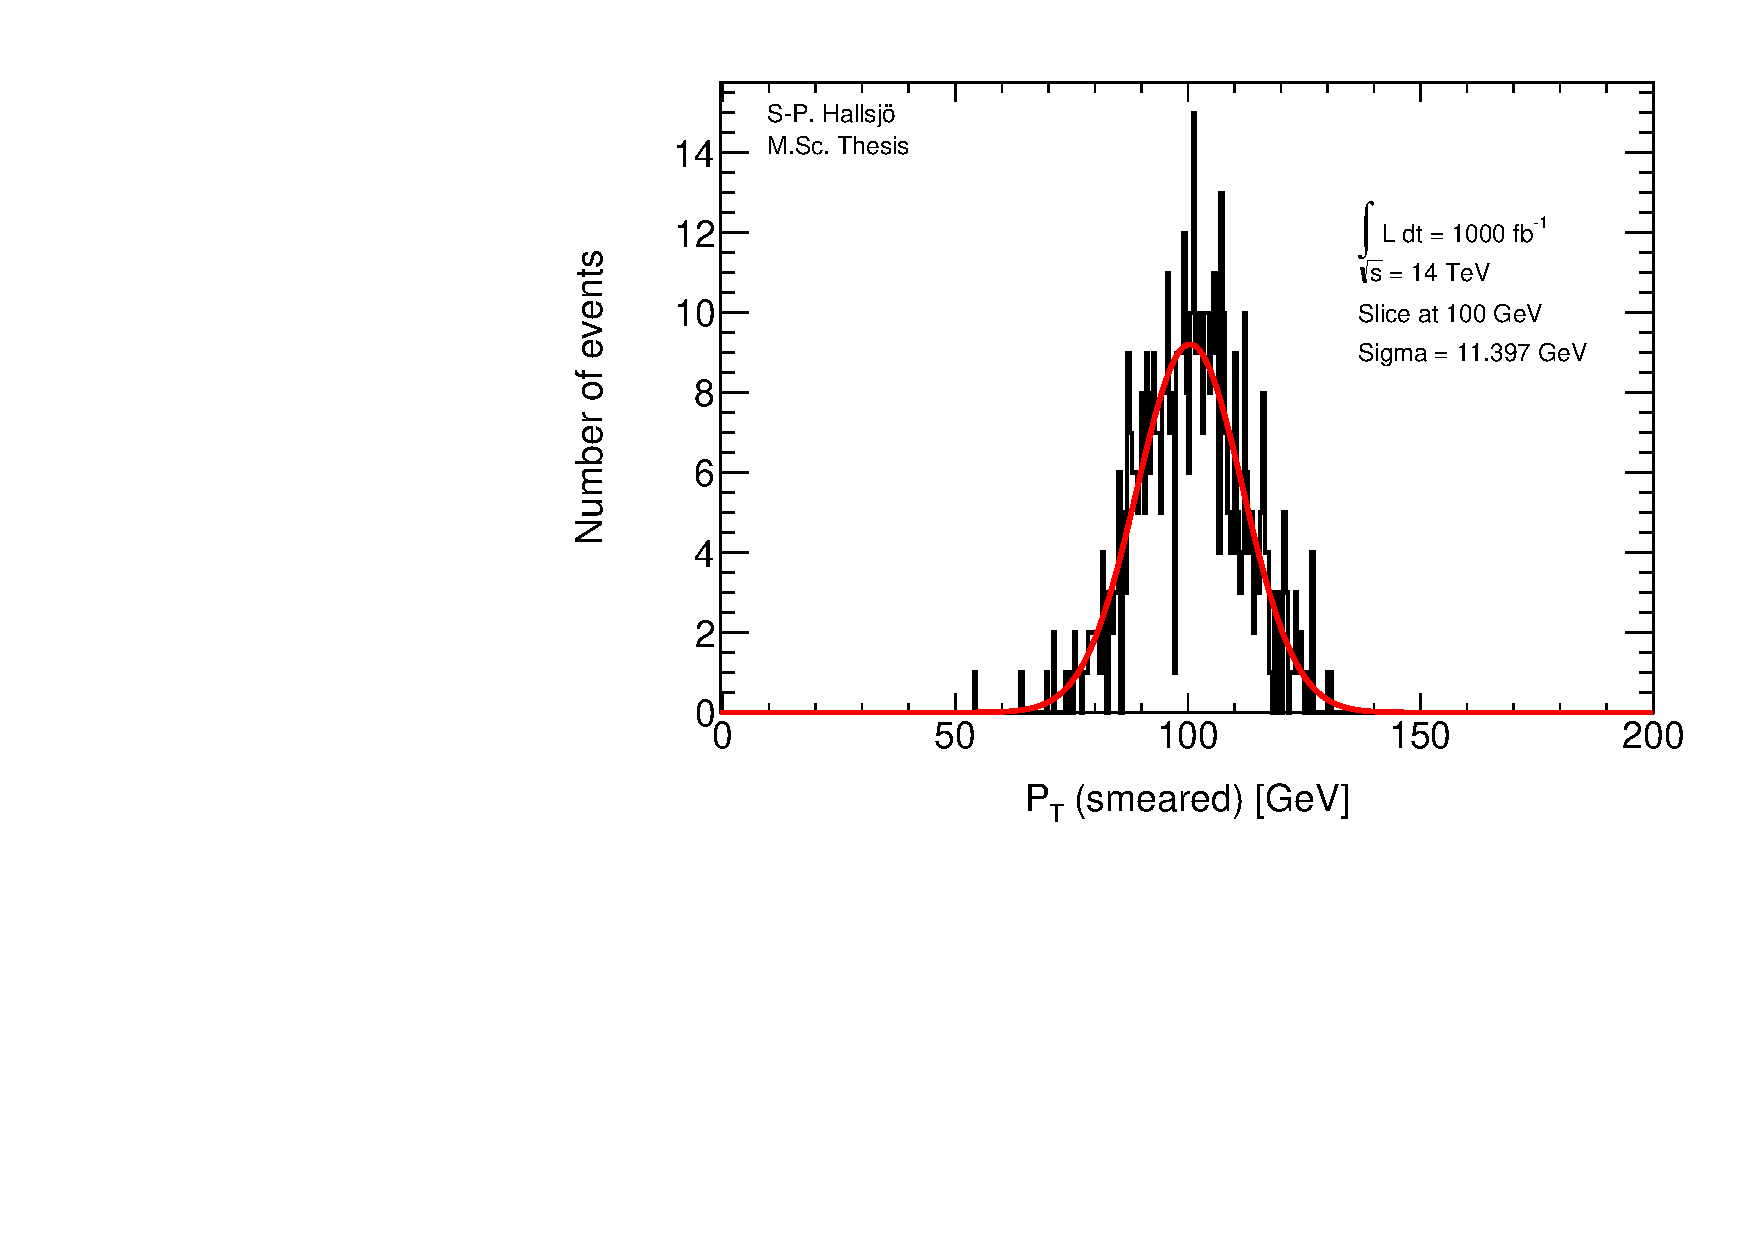
\includegraphics[width=0.5\textwidth]{jeteta1.pdf}
    }
    \hfill
\subfloat[Jet smearing for $0.8<\abs{\eta}<1.2$.\label{fig:jet:2}]{%
      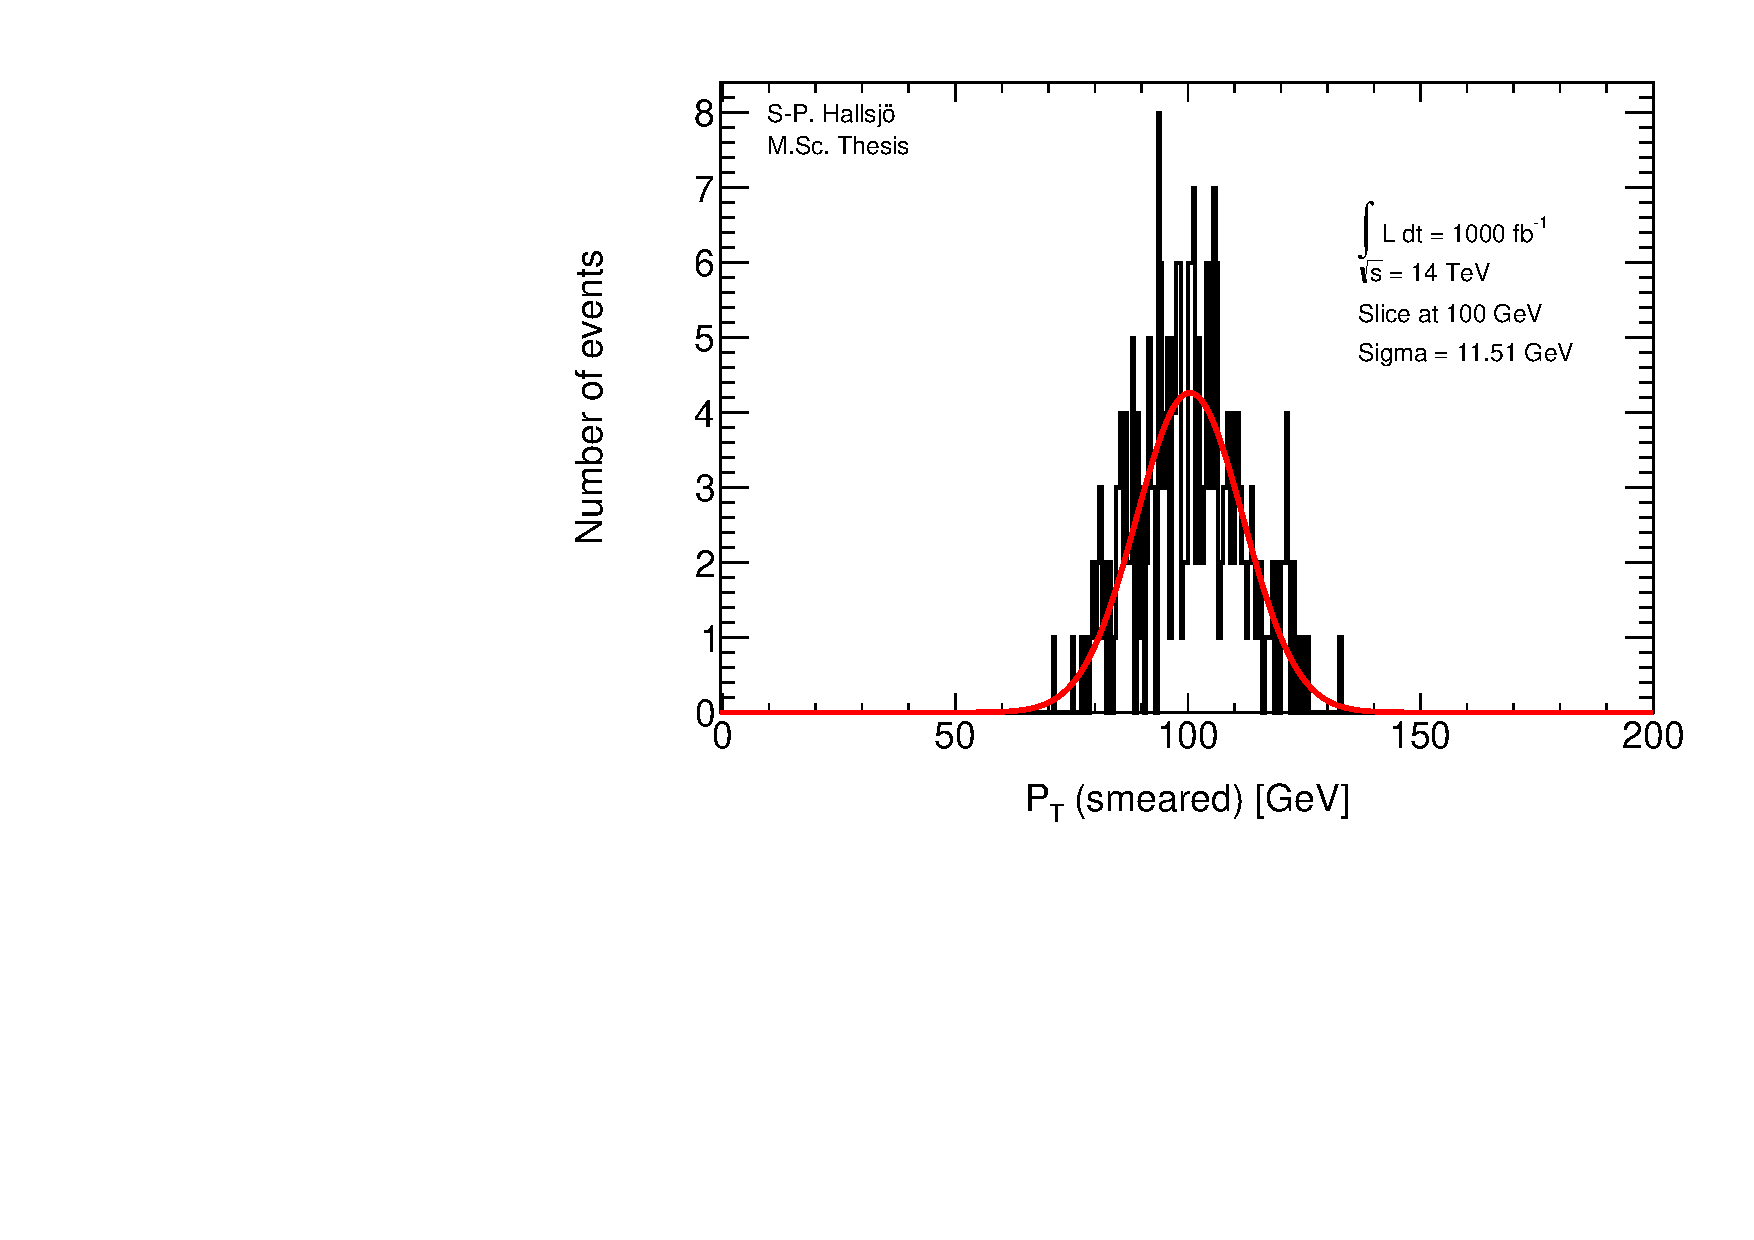
\includegraphics[width=0.5\textwidth]{jeteta2.pdf}
    }
    \hfill
        \subfloat[Jet smearing for $1.2<\abs{\eta}<2.8$. \label{fig:jet:3}]{%
     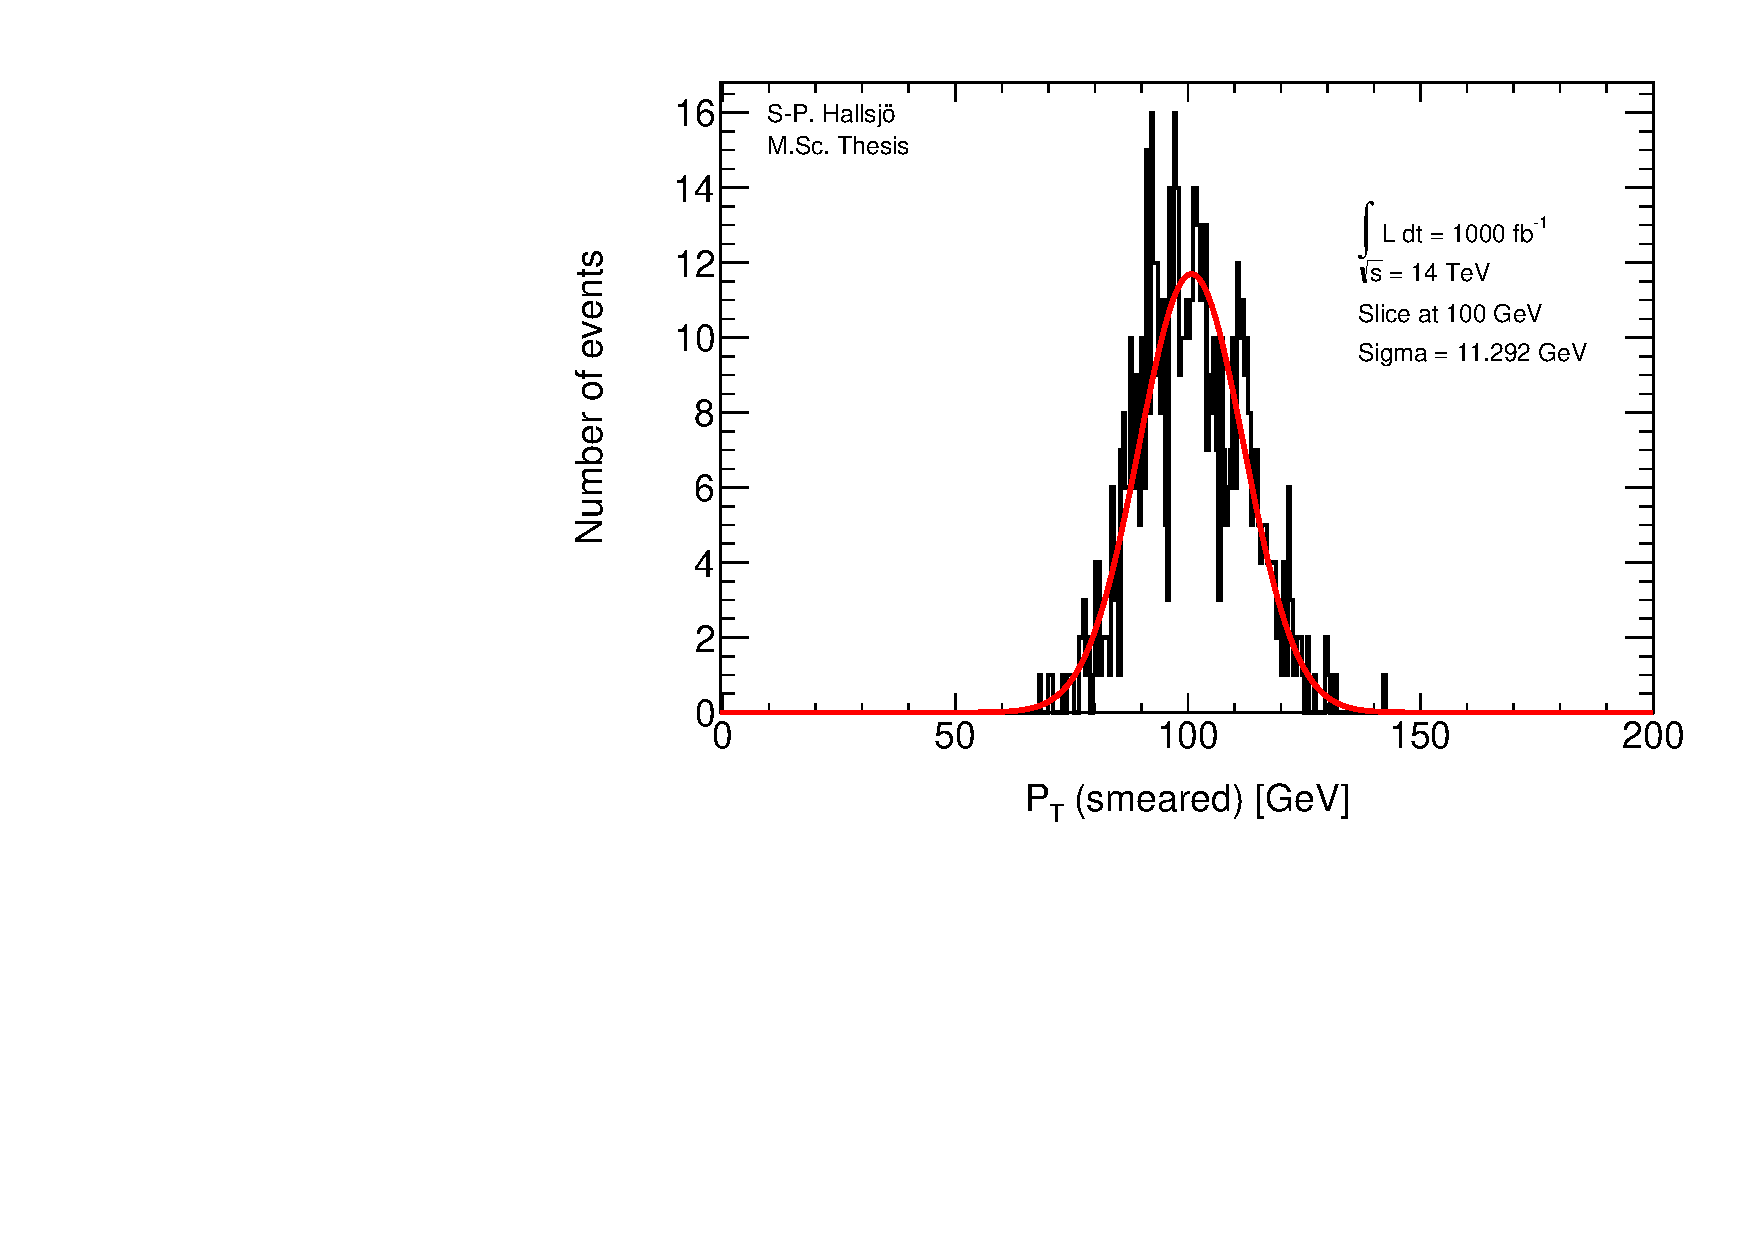
\includegraphics[width=0.5\textwidth]{jeteta3.pdf}
    }
    \hfill
\subfloat[Jet smearing for $2.8<\abs{\eta}<3.6$. \newline Very odd due to the low amount of available data. \label{fig:jet:4}]{%
      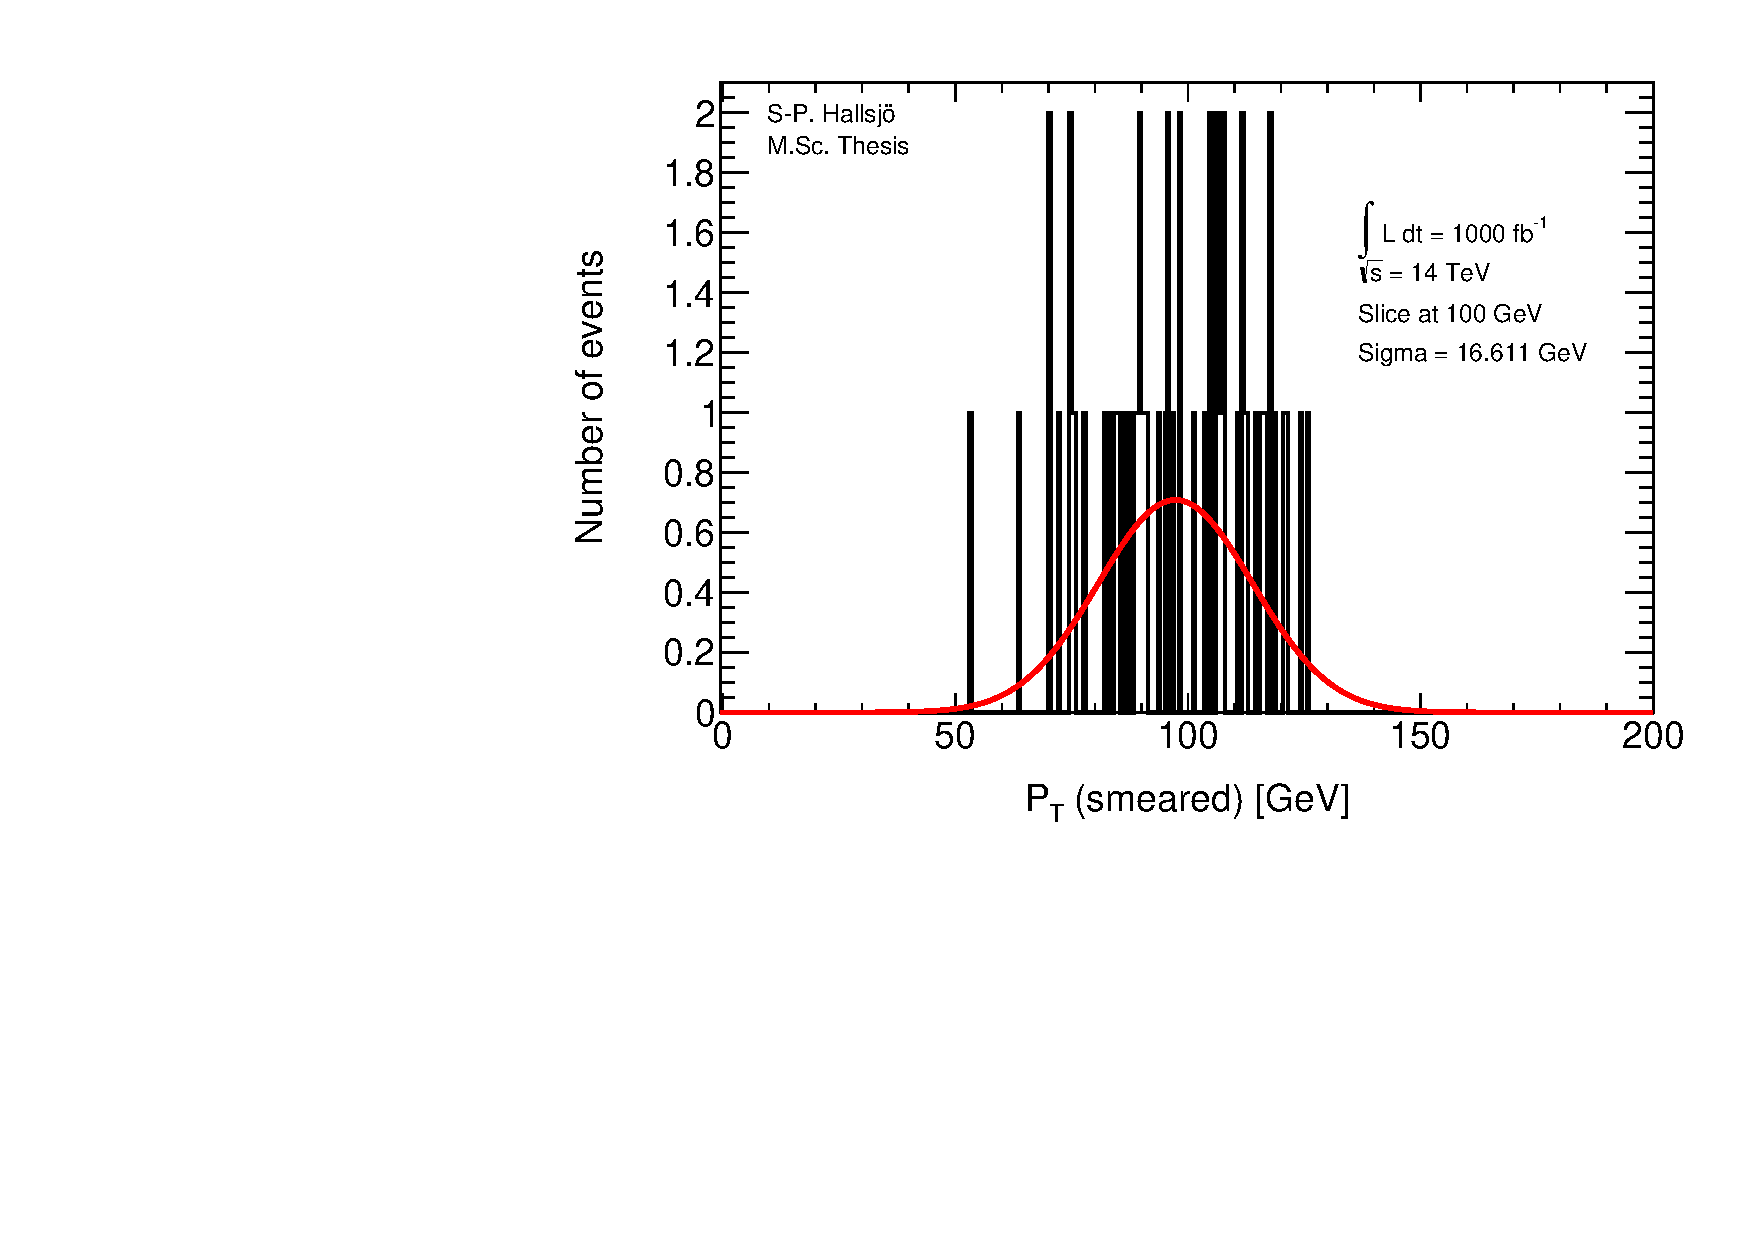
\includegraphics[width=0.5\textwidth]{jeteta4.pdf}
    }
        \hfill
\subfloat[Jet smearing for $\abs{\eta}<0.8$ at $\obs{\mu}=140$. \label{fig:jet:5}]{%
      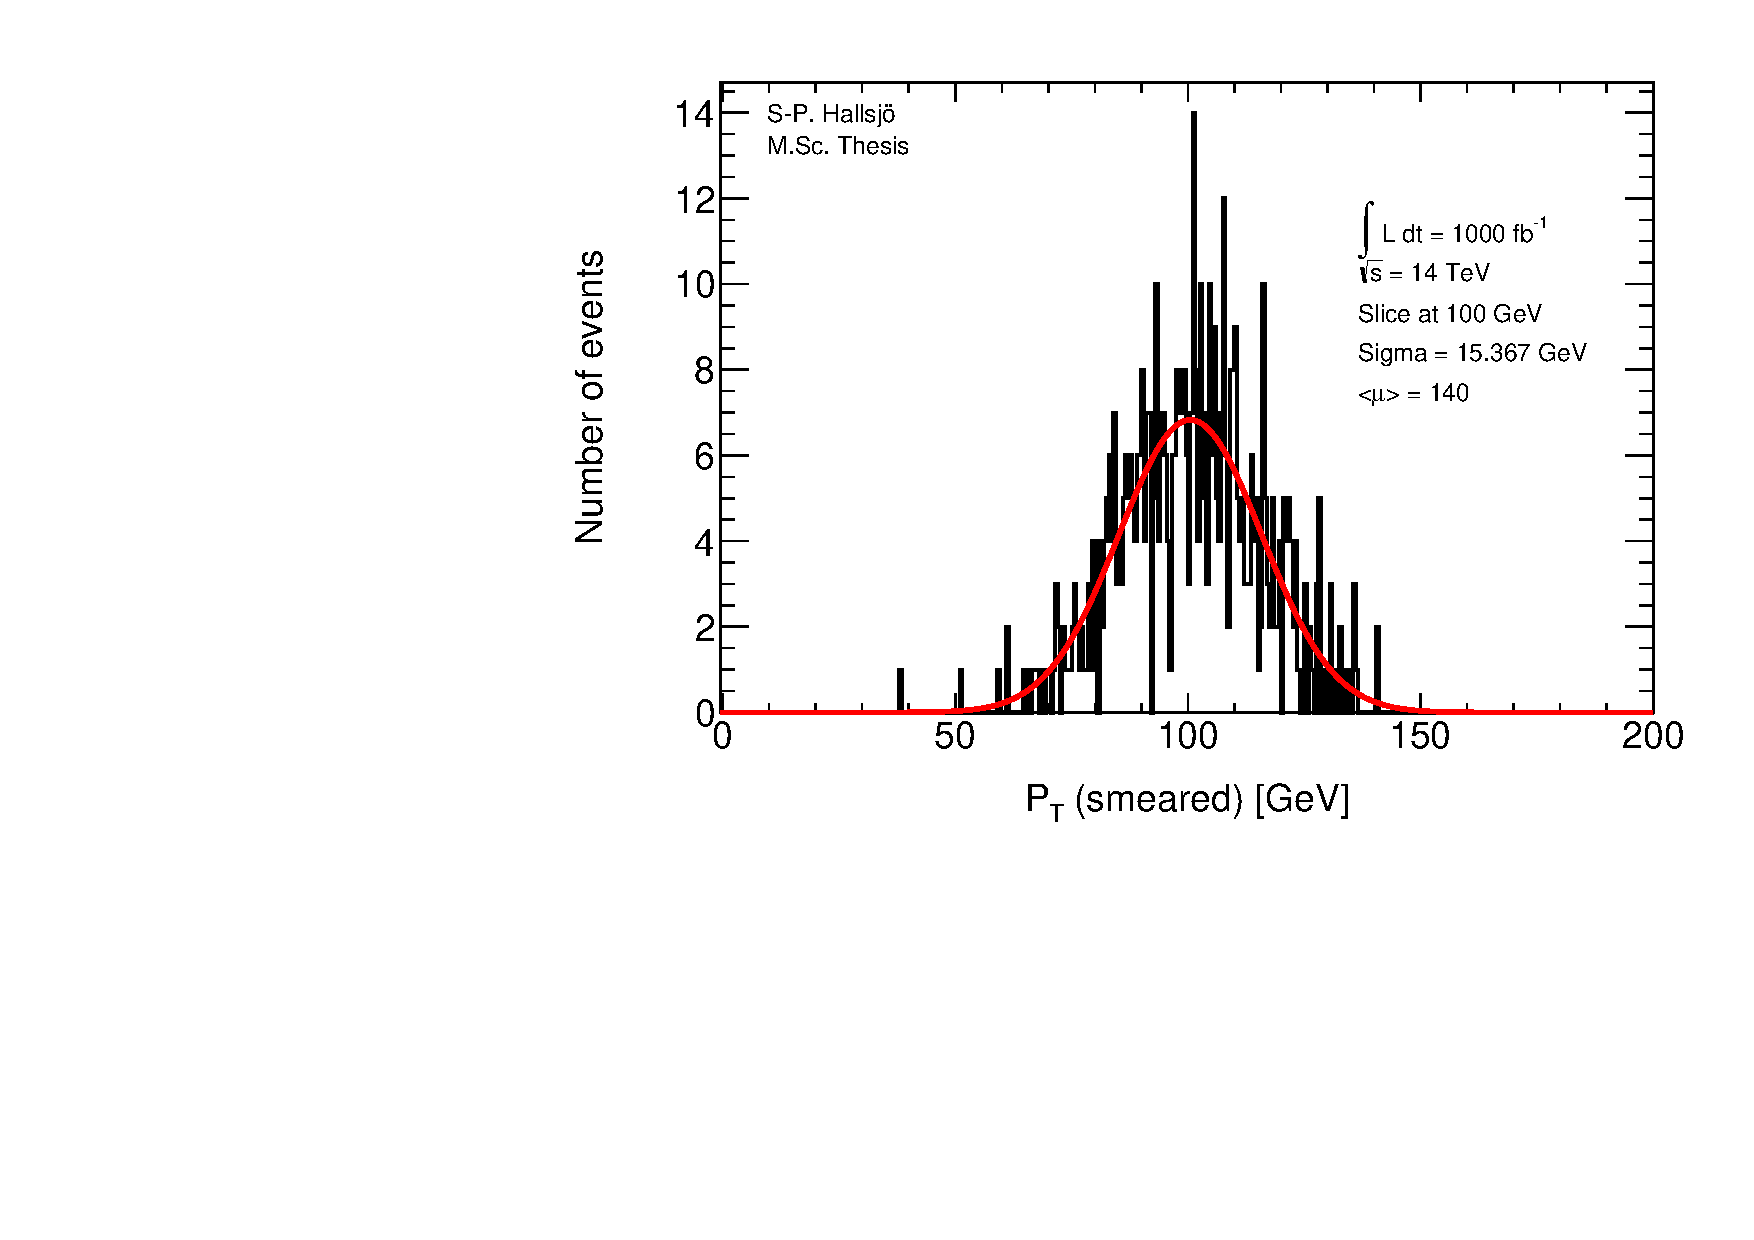
\includegraphics[width=0.5\textwidth]{jeteta1140.pdf}
    }
            \hfill
\subfloat[Jet smearing for $0.8<\abs{\eta}<1.2$ \newline at $\obs{\mu}=140$. \label{fig:jet:6}]{%
      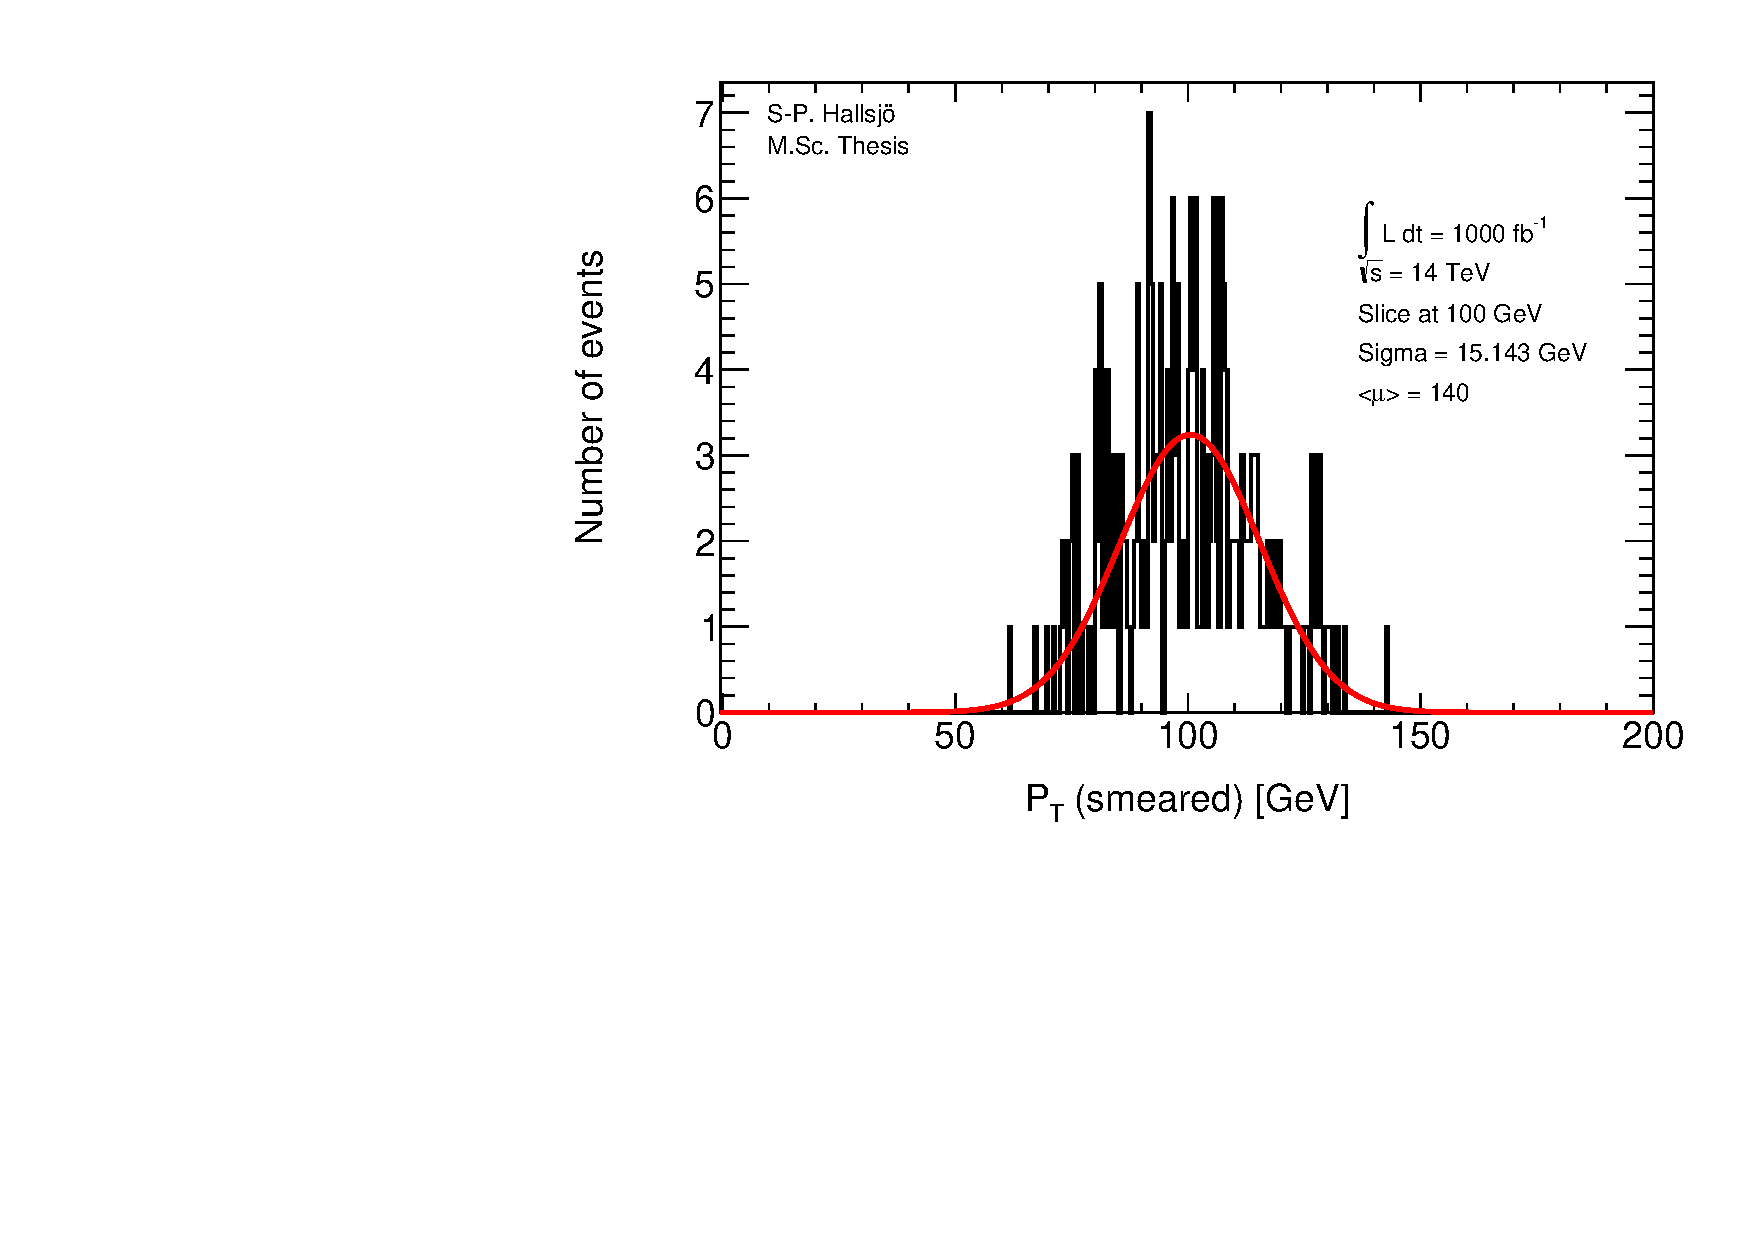
\includegraphics[width=0.5\textwidth]{jeteta2140.pdf}
    }
    \caption{Jet smearing plots.}
    \label{fig:jet}
\end{figure}

\newpage
\subsection{Missing Transversal Energy}
These figures are given as smeared value from origin, thus at 0 it represents that the energy is unsmeared, compared to the others where the slice value represents the unsmeared.

Here the $E_T^{Miss}$ is projected down to the x- and y-axis, since these are the transversal axes, to be smeared. 
 \begin{figure}[H] %!ht
    \subfloat[$E_T^{Miss}$ smearing along the x-axis. \label{fig:MET:x}]{%
     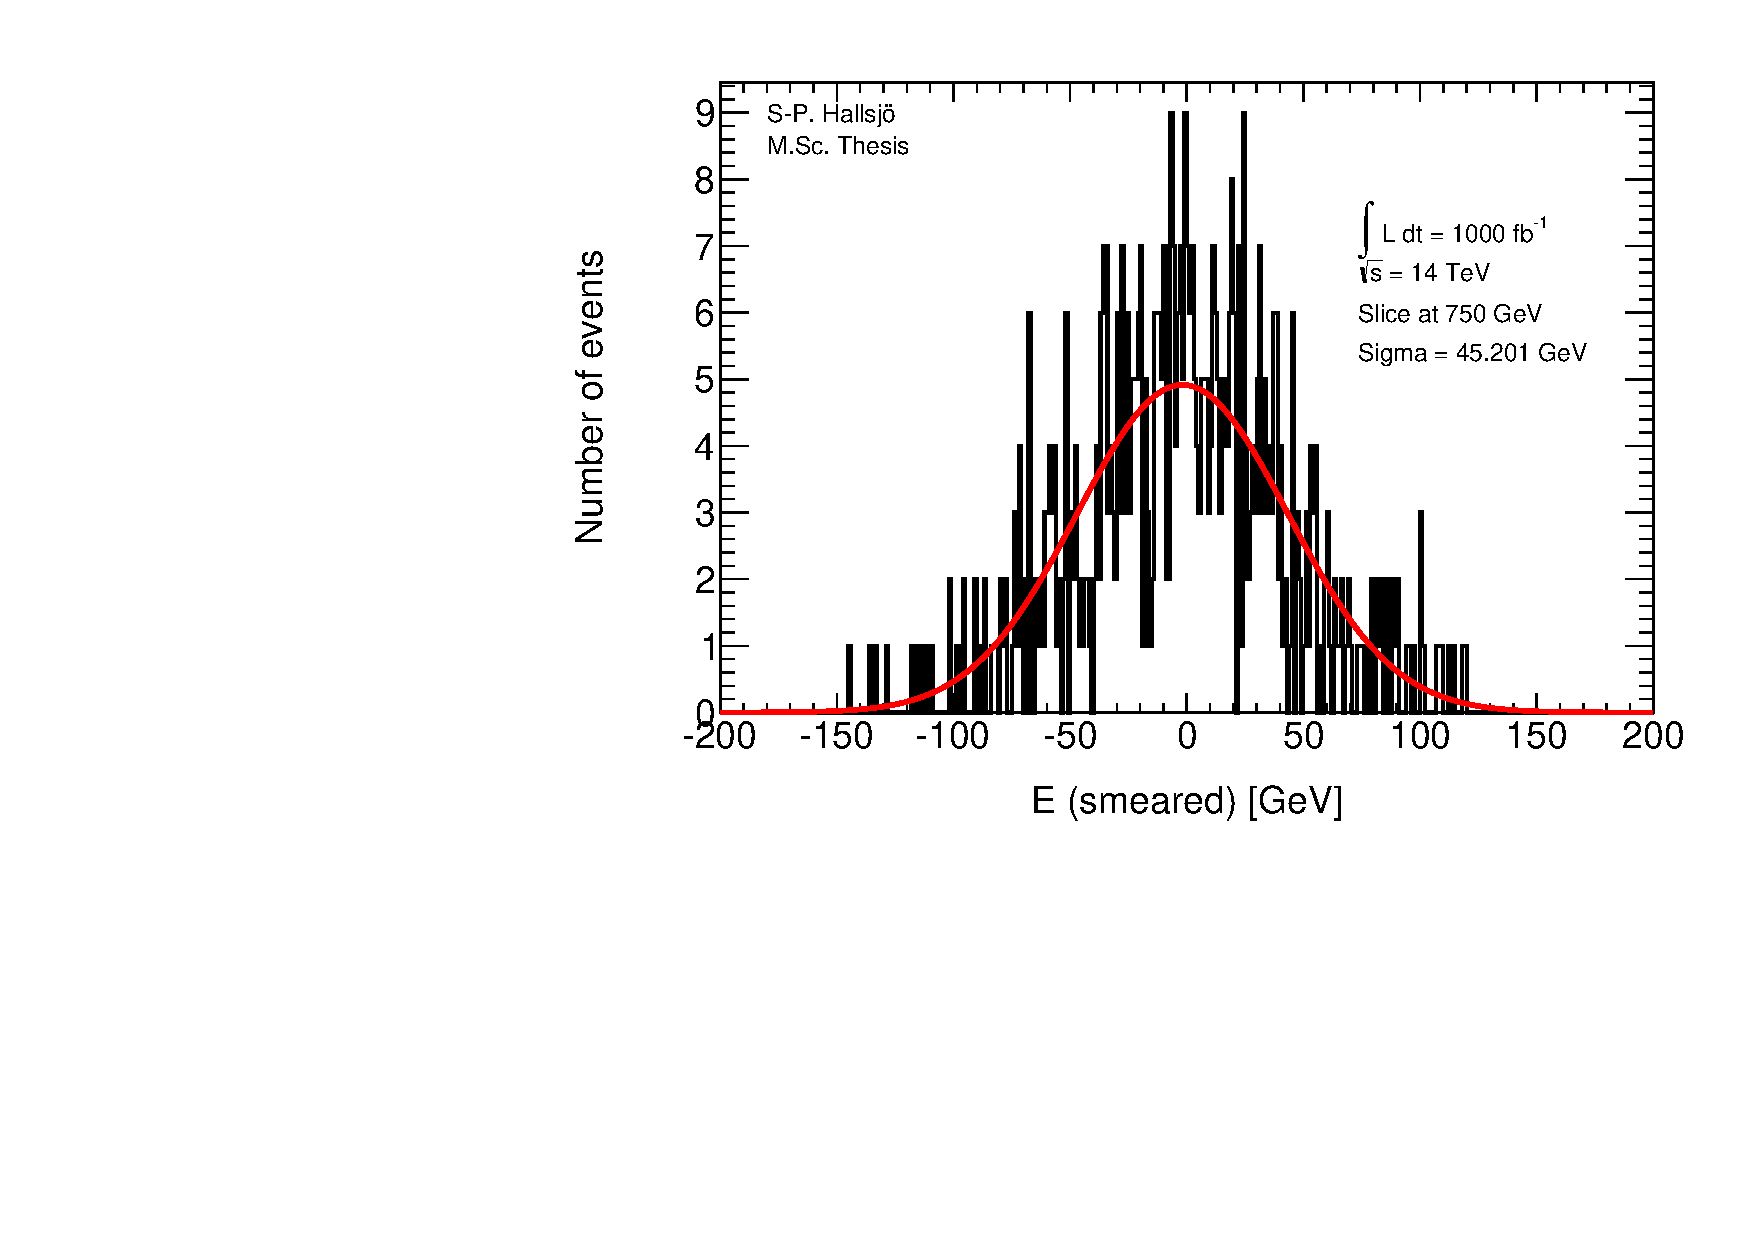
\includegraphics[width=0.5\textwidth]{METx.pdf}
    }
    \hfill
    \subfloat[$E_T^{Miss}$ smearing along the y-axis.\label{fig:MET:y}]{%
      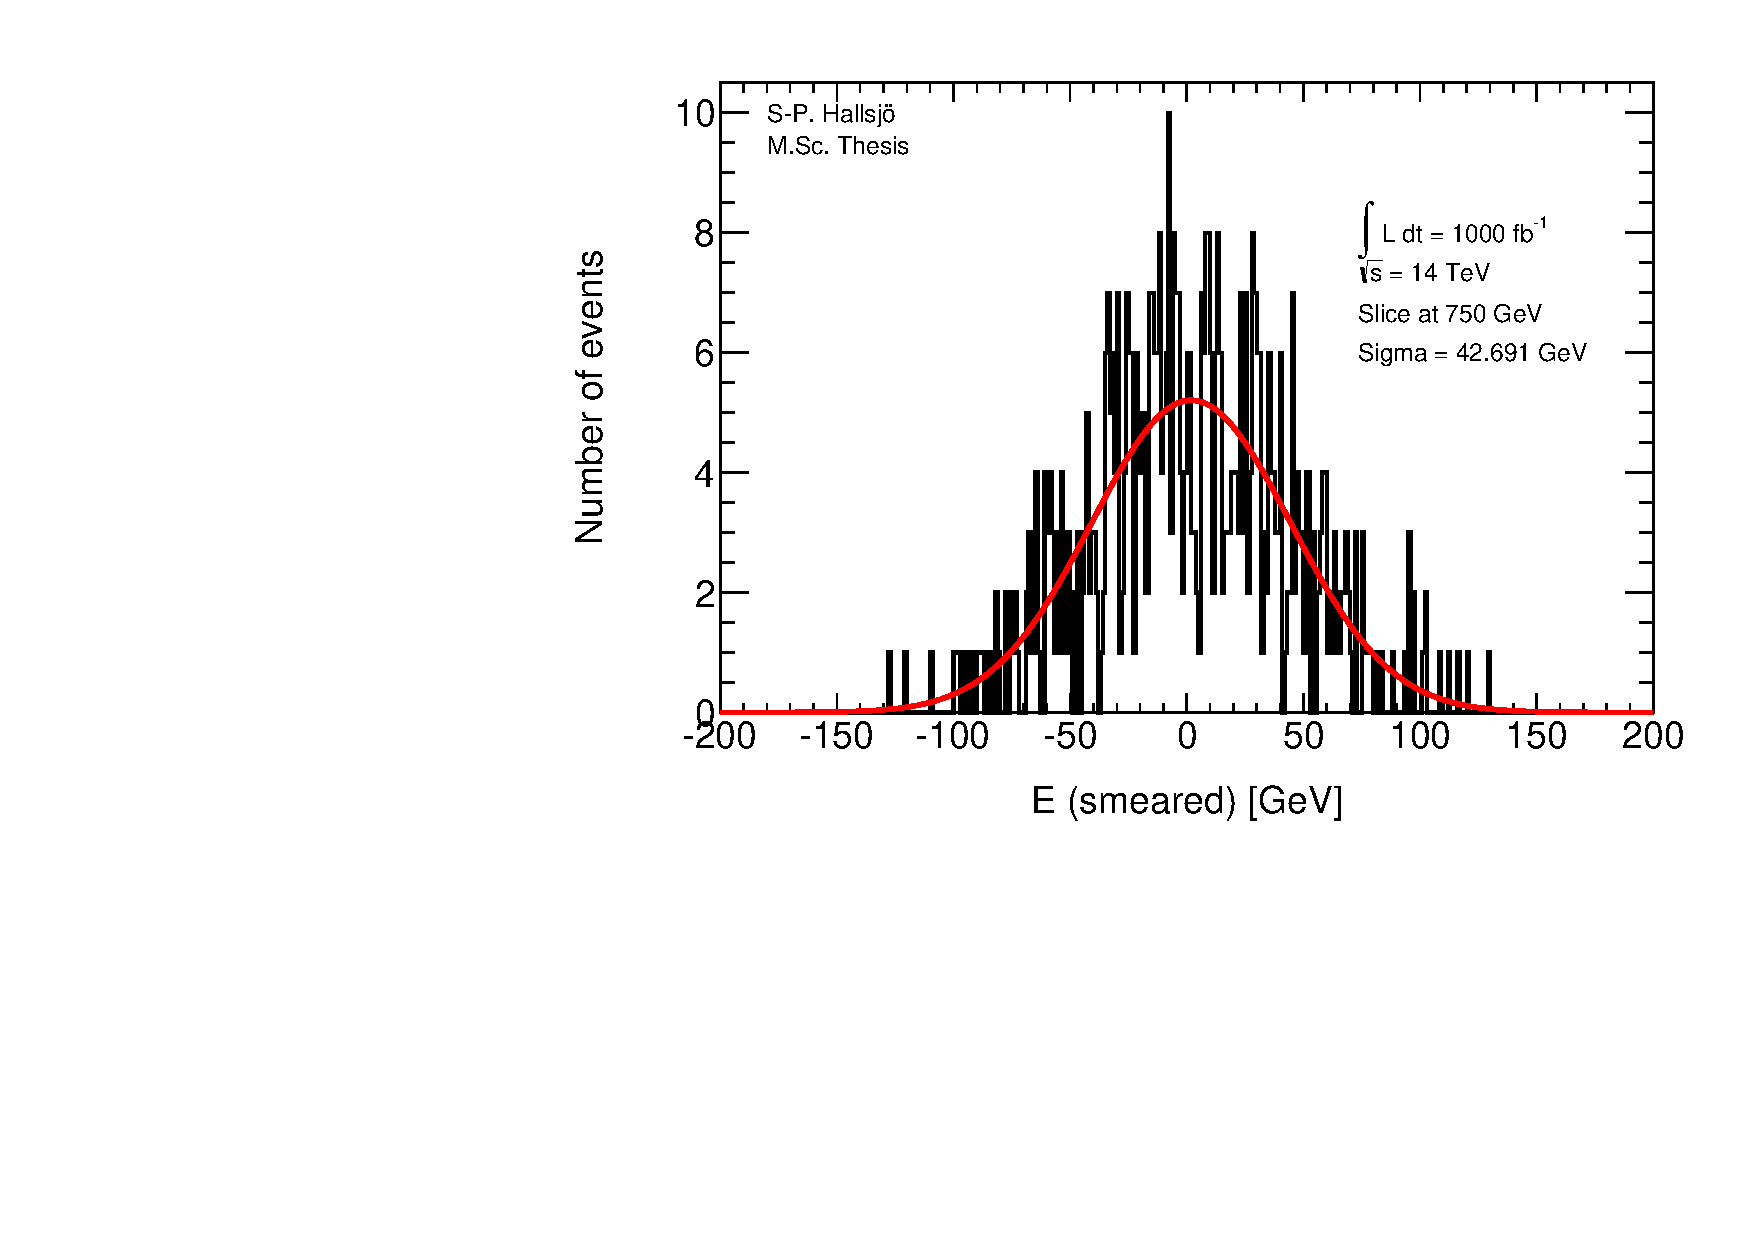
\includegraphics[width=0.5\textwidth]{METy.pdf}
    }
        \hfill
    \subfloat[$E_T^{Miss}$ smearing along the y-axis for $\obs{\mu}=140$.\label{fig:MET:140}]{%
      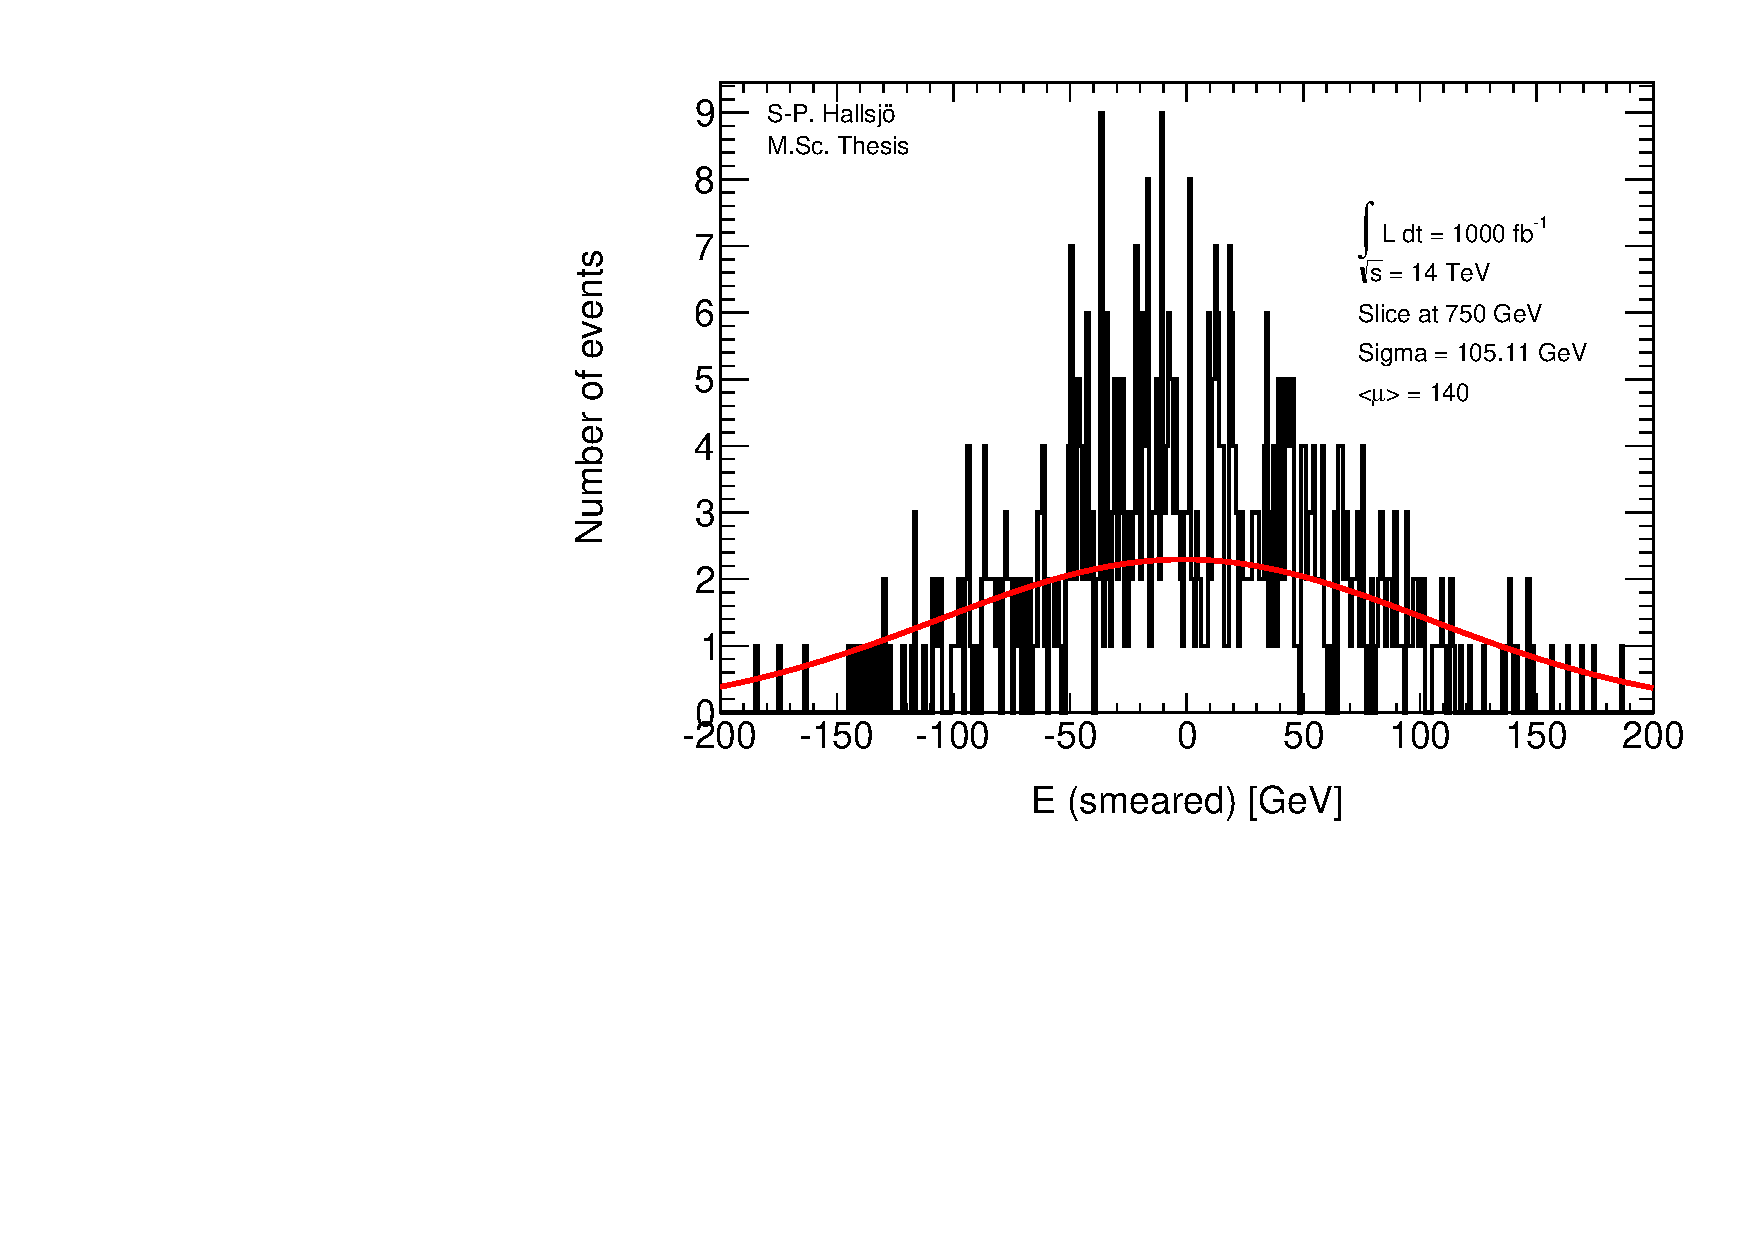
\includegraphics[width=0.5\textwidth]{mety140.pdf}
    }
   \caption{$E_T^{Miss}$ smearing plots}
    \label{fig:MET}
  \end{figure}
\newpage
\section{Expected results}\label{cha:vali:sec:expr}

The expected response has been calculated and taken from \citep{ATL-PHYS-PUB-2013-004}.

The independence of pile-up for leptons and photons is backed up in previous research, for instance \citep{Electronperf:2011, ATLAS:LOI2} were the first states:
\begin{quotation}
``The uncertainty due to pile-up was investigated by comparing simulated MC samples with and without pile-up and was found to be negligible''
\end{quotation}


To validate the smearing code comparisons were made with \citep{ATL-PHYS-PUB-2013-004} which gave the following formulation for the expected $\sigma$: 
\begin{table}[H]
\renewcommand{\arraystretch}{1.5} %Change height of tabel
\begin{center}
\begin{tabular}{|l|l|}
\hline
Observable & Absolute $\sigma$ \\ \hline
Electron \& photon & $\sigma=0.3\oplus 0.1\sqrt{E(GeV)}\oplus 0.01E(GeV)$, $|\eta|<$ 1.4 \\
& $\sigma=0.3\oplus 0.15\sqrt{E(GeV)}\oplus 0.015E(GeV)$, 1.4 $<|\eta|<$ 2.47 \\ \hline 
Muon momentum& $\sigma=\frac{\sigma_{id} \sigma_{ms}}{\sigma_{id} \oplus \sigma_{ms}}$\\
& $\sigma_{id}=P_T(a_1 \oplus a_2 P_T)$\\
& $\sigma_{ms}=P_T(\frac{b_0}{P_T} \oplus b_1 \oplus b_2 P_T)$\\ \hline
Tau energy& $\sigma =(0.03\oplus \frac{0.76}{\sqrt{E(GeV)}})E(GeV)$, for 3 prong.\\ \hline
Jet momentum& $\sigma = P_T(GeV)(\frac{N}{P_T} \oplus \frac{S}{\sqrt{P_T}} \oplus C)$ \\ 
& where $N=a(\eta)+b(\eta)\mu$ \\ \hline
$E_T^{Miss}$ & $\sigma = (0.4+0.09\sqrt{\mu})\sqrt{\sum E(GeV)+20\mu}$ \\ \hline
\end{tabular}
\end{center}
\renewcommand{\arraystretch}{1.0} %Change back
\caption{Expected absolute $\sigma$ where the parameters are given for muons in \tableref{tab:muonparam} and for jets in \tableref{tab:jetparam}. Functions take from \citep{ATL-PHYS-PUB-2013-004}.}
\label{tab:expected sigma}
\end{table}
%\begin{itemize}
%\item For muon: Where a$_i$ and b$_i$ are dependent on $\eta$.
%\item For muon: All parameters are given in \tableref{tab:muonparam}.
%\item For tau: Fixed at 3 prong. 1 prong exists though was not used in this thesis. \\
%Where prong refers to the different amount of tracks that from which they were reconstructed.
%\item For Jet: Where N, S, and C depend on $\eta$. N is also dependent on the pile-up that is simulated.\\
%\item For jet: All parameters are given in %\tableref{tab:jetparam} where $N=a(\eta)+b(\eta)\mu$.
%Where $\eta$ is the same as discussed in \subsectionref{sec:eo:subsec:coord}
%\item All parameters can be found in \citep{ATL-PHYS-PUB-2013-004}.
%\end{itemize}

\begin{table}[H]
\renewcommand{\arraystretch}{1.5} %Change height of tabel
\begin{center}
\begin{tabular}{|l|l|l|l|l|l|}
\hline
 &$a_1$&$a_2$&$b_0$&$b_1$&$b_2$ \\ \hline
$\abs{\eta}<1.05$&0.01607&0.000307&0.24&0.02676&0.00012 \\ \hline
$\abs{\eta}>1.05$&0.03000&0.000387&0.00&0.03880&0.00016 \\ \hline
\end{tabular}
\end{center}
\caption{Parameters used in the muon smearing function taken from \citep{ATL-PHYS-PUB-2013-004}.}
\label{tab:muonparam}
\renewcommand{\arraystretch}{1.0} %Change back
\end{table}
\begin{table}[H]
\renewcommand{\arraystretch}{1.5} %Change height of tabel
\begin{center}
\begin{tabular}{|l|l|l|l|l|}
\hline
$\abs{\eta}$&a&b&S&C \\ \hline
0-0.8&3.2&0.07&0.74&0.05 \\
0.8-1.2&3.0&0.07&0.81&0.05 \\
1.2-2.8&3.3&0.08&0.54&0.05 \\
2.8-3.6&2.8&0.11&0.83&0.05 \\ \hline
\end{tabular}
\end{center}
\caption{Parameters used in the jet smearing function taken from \citep{ATL-PHYS-PUB-2013-004}.}
\label{tab:jetparam}
\renewcommand{\arraystretch}{1.0} %Change back
\end{table}

\begin{table}[H]
\begin{center}
\begin{tabular}{|l|l|l|}
\hline
Process&$\sigma$ [GeV]&Expected $\sigma$\\ \hline
Electron low $\eta$&$1.24948 \pm 0.0481987$&1.18427\\
High $\eta$&$1.8211 \pm 0.141329$&1.74446\\ \hline
Photon low $\eta$&$1.18986 \pm 0.0400187$&1.18427\\
High $\eta$&$1.80297 \pm 0.0374312$&1.744463\\ \hline
Muon low $\eta$&$1.19016 \pm 0.0524938$&1.49789\\
High $\eta$&$1.70694 \pm 0.0882606$&2.18318\\ \hline
Tau&$10.8992 \pm 0.299761$&10.3388\\ \hline
Jet low $\eta$&$11.3974 \pm 0.351391$&11.5983\\
$\obs{\mu}=140$&$15.3673 \pm 0.473783$&15.7721\\
Mid low $\eta$&$11.5096 \pm 0.518872$&11.9352\\
$\obs{\mu}=140$&$15.1427 \pm 0.682649$&15.9515\\
Mid high $\eta$&$11.2916 \pm 0.310314$&10.9439\\
High $\eta$&$16.6112 \pm 1.52891$&13.5\\ \hline
$E_T^{Miss} $x$-$axis&$45.2013 \pm 1.35426$&48.4483\\ \hline
$E_T^{Miss} $y$-$axis&$42.6906 \pm 2.27904$&48.44834\\ 
$\obs{\mu}=140$&$105.109 \pm 12.239$&87.2812\\  \hline
\end{tabular}
\end{center}
\caption{$\sigma$ values.}
\label{tab:sigmaval}
\end{table}
\begin{itemize}
\item Where the given $\sigma$ is still the absolute. 
\item Where the large difference between calculated and expected $\sigma$ for Muons and $E_T^{Miss}$ is explained by incorrectly calculated errors in $\sigma$.  
\end{itemize}
\newpage
\section{Discussion}
\subsection{Smearing independent on pile-up}\label{chap:vali:sec:dis:subsec:smearindep}
From the validation done it was interesting to note that the smearing functions were created from previous studies, \citep{Electronperf:2011, ATLAS:LOI2}, which had shown that leptons and photons are not affected by pile-up.
This may seem incredible however it becomes quite logical when one understands how the detectors work. To be able to detect particles the detectors must detect an excess of energy which comes from a particle passing through. This should not be distorted by an increased pile-up. The amount of particles passing through will of course increase, but the detections should be unaffected as well as the recreation of the events. However with the same logic it makes sense that jets and $E_T^{Miss}$ are quite affected since they are combined of several parts, either hadronic particles or by all the transversal missing energy. 

Another interesting part is how the effect diminishes with and increasing energy. As seen above, and through the the formula, for the high energies which were of interest here the effect is minimal. 
\subsection{Comparison to expected results}
One of the major problems in the comparison was to get the significance of the Gaussian fit to be calculated correctly. The tool ROOT has a lot of different features which made this task somewhat difficult. Also since this is a statistical property there is a statistical fluctuation in the result. 

Another was to retrieve the correct values from the paper, \citep{ATL-PHYS-PUB-2013-004}, since it was unclear if the values given were absolute or scale dependent. This has now been corrected in a new version of the paper.
\newpage
\section{Conclusion}
The smearing functions work as intended within 5.8 sigma, however when using a test box and averaging the sigmas one ends up with half of this for the extreme cases, muons and $E_T^{Miss} $y$-$axis.